\documentclass[11pt]{article}
\usepackage[T1]{fontenc}
\usepackage[utf8]{inputenc}
\usepackage{lmodern}
\usepackage[margin=1in]{geometry}
\usepackage{amsmath,amssymb,amsthm,mathtools}
\usepackage{enumitem,booktabs,microtype,needspace}
\usepackage{tikz}
\usepackage[numbers,sort&compress]{natbib}
\usepackage{xurl}
\usepackage[hidelinks,breaklinks]{hyperref}
\hypersetup{
  pdftitle={Continuous Phase Foliations Create Analytic Caustic Collars},
  pdfauthor={OpenAI},
  pdfsubject={Near-boundary billiard rigidity from continuous invariant phase foliations}
}
\newcommand{\R}{\mathbb{R}}
\newcommand{\C}{\mathbb{C}}
\newcommand{\T}{\mathbb{T}}
\newcommand{\ii}{\mathrm{i}}
\newcommand{\dd}{\mathop{}\!\mathrm{d}}
\newcommand{\eps}{\varepsilon}
\newcommand{\cS}{\mathcal{S}}
\newtheorem{theorem}{Theorem}[section]
\newtheorem{lemma}[theorem]{Lemma}
\newtheorem{proposition}[theorem]{Proposition}
\newtheorem{corollary}[theorem]{Corollary}
\theoremstyle{definition}
\newtheorem{definition}[theorem]{Definition}
\theoremstyle{remark}
\newtheorem{remark}[theorem]{Remark}
\numberwithin{equation}{section}
\setlist{itemsep=3pt,topsep=5pt}
\setlength{\emergencystretch}{2em}
\title{Continuous Phase Foliations Create Analytic Caustic Collars}
\author{OpenAI}
\date{September 24, 2026}

\begin{document}
\maketitle

\begin{abstract}
For a smooth strictly convex planar billiard of positive curvature, a
continuous foliation of a full grazing annulus by individually invariant
essential curves forces an analytic boundary and a jointly analytic collar
of smooth strictly convex caustics. The physical-collar rigidity theorem
proved in the companion article then implies that the table is an ellipse.
\end{abstract}

\section{Introduction}\label{sec:introduction}

Let \(\Omega\subset\R^2\) be a bounded strictly convex open set whose
boundary is a \(C^\infty\) simple closed regular curve with positive
curvature. Orient the boundary counterclockwise, write its arclength
coordinate as \(s\in\R/L\mathbb Z\), and let \(\delta\in(0,\pi)\) be the
angle of the outgoing velocity measured counterclockwise from the
positive tangent. Reflection at a boundary point with outward unit
normal \(n\) sends an incoming velocity \(v\) to
\(v-2(v\cdot n)n\). The resulting billiard map \(T\) acts on
\[
M=(\R/L\mathbb Z)\times(0,\pi),
\]
and \(\delta\downarrow0\) is the grazing end considered below.
Write \(\T=\R/2\pi\mathbb Z\) for the angular circle.

\begin{theorem}[Phase-foliation rigidity]\label{thm:main}
Suppose a \(T\)-invariant open annulus \(U\subset M\) contains
\((\R/L\mathbb Z)\times(0,\eta)\) for some \(\eta>0\).
Suppose there is a homeomorphism
\[
H:\mathbb S^1\times(0,1)\longrightarrow U
\]
whose leaves are essential simple closed curves, each individually
invariant under \(T\). Then \(\Omega\) is an ellipse: there are
\(c\in\R^2\) and a real symmetric positive-definite matrix \(Q\) such that
\[
\Omega=\{x\in\R^2:(x-c)^TQ(x-c)<1\}.
\]
Circles are included.
\end{theorem}

For an elliptical table, the confocal elliptic caustics give such a
grazing foliation \citep{Lazutkin1973}; for a circular table, the
corresponding caustics are concentric circles.
Only continuity of the leaves and of their transverse dependence is
assumed. The foliation need not extend to the rest of the phase cylinder,
and the width \(\eta\) may be arbitrarily small. The main issue is that a
continuous essential phase curve need not initially be given as the
tangent lines of a smooth convex caustic.

The complete companion article \emph{Rigidity of Smooth Billiards with a
Continuous Caustic Collar} \citep{NB} supplies three analytic inputs and
the final physical-collar rigidity theorem. Its stationary-mesh and
Fourier-row estimates apply to arbitrary normalized actions; its buffered
division lemma is an analytic estimate. Their precise hypotheses are
recalled at the points of use. Here we establish the additional dynamical
and geometric steps needed to apply them to a merely continuous phase
foliation. In particular, we construct the physical collar before invoking
the companion's ellipse theorem.

\subsection{Context and significance}

The Birkhoff conjecture asks whether an integrable strictly convex planar
billiard must be an ellipse. Birkhoff developed the convex billiard as a
dynamical model \citep{Birkhoff1927}; Poritsky's early printed formulation
also studied compatible string constructions, under hypotheses stronger
than a foliation alone \citep{Poritsky1950}. The distinction between a
full foliation and a family with gaps is essential. Lazutkin's theorem
guarantees a Cantor family of near-boundary invariant curves for
sufficiently smooth positively curved tables, rather than a full foliation
\citep{Lazutkin1973}. Marvizi and Melrose constructed a grazing first
integral modulo a flat error, not an exact invariant foliation
\citep{MarviziMelrose1982}. Positive curvature is substantive: Mather
excluded grazing caustics when boundary curvature vanishes
\citep{Mather1982}.

Stronger or different integrability hypotheses give complementary
rigidity results. Bialy proved that foliation of the entire phase
cylinder by noncontractible invariant circles forces a circle
\citep{Bialy1993}. Avila, De Simoi, and Kaloshin proved local rigidity
near small-eccentricity ellipses \citep{ADK2016}, and Kaloshin and
Sorrentino treated perturbations of ellipses of arbitrary eccentricity
\citep{KS2018}. Bialy and Mironov allowed a continuous phase foliation
under central symmetry when the foliated region reaches the invariant
four-periodic curve \citep{BialyMironov2022}. Koval's local strong
result treats caustics at all rational rotations in an arbitrarily small
interval above zero, under closeness to almost every ellipse and
high-regularity bounds
\citep{Koval2026}. These results impose geometric restrictions or require
invariant curves extending beyond an arbitrarily thin grazing annulus.

Birkhoff's invariant-curve theorem for twist maps explains why graphs are
the natural intermediate objects \citep{Arnaud2009}. Here the initial
leaves are only continuous essential curves, and the entire annulus is
foliated. We therefore prove graphness directly from both billiard twist
signs and finite-area recurrence. The full collar then supplies a wholly
periodic graph at every sufficiently small rational rotation. The
stationary actions of those graphs yield high-frequency equations for the
boundary. First-order Fourier obstructions for rational caustics in
perturbations of the circle were developed by \citet{RamirezRos2006};
quantitative constraints near ellipses appear in \citet{ADK2016}.
The analytic inversion here uses the companion's arbitrary-input estimates
without a perturbative assumption.

Together with the physical-collar rigidity theorem of \cite{NB},
Theorem~\ref{thm:main} resolves the near-boundary Birkhoff conjecture
positively in the continuous phase-foliation formulation above.
The additional point established here is the passage from merely
continuous invariant phase leaves to the smooth physical caustic
hypothesis. This passage requires neither a symmetry assumption nor
closeness to a circle or ellipse.

\subsection{The regularity reduction}

A \emph{smooth convex caustic} is a \(C^\infty\) simple closed regular
curve in \(\Omega\), bounding a strictly convex set, such that a billiard
segment tangent to it remains tangent after reflection at either
endpoint. A \emph{continuous physical caustic collar} is a relatively
open set \(A\subset\overline\Omega\), containing \(\partial\Omega\),
together with a homeomorphism
\[
H_0:\mathbb S^1\times[0,1)\longrightarrow A
\]
whose zero leaf is \(\partial\Omega\) and whose positive leaves are smooth
convex caustics. This is the hypothesis of the following companion theorem.

\begin{theorem}[Physical-collar rigidity,
  {\citep[Definition~1.1 and Theorem~1.2]{NB}}]
\label{thm:nb-rigidity}
A bounded strictly convex planar domain with \(C^\infty\) regular boundary
of positive curvature and a continuous physical caustic collar is an
ellipse.
\end{theorem}

The core reduction proved below is stronger than the smoothness needed
for this application.

\begin{theorem}[Regularity of a phase-foliated collar]
\label{thm:collar-regularity}
Under the hypotheses of Theorem~\ref{thm:main}, the boundary is real
analytic. There are \(\lambda_0>0\) and a jointly real-analytic map
\[
\Gamma:\mathbb T\times[0,\lambda_0]\longrightarrow\R^2
\]
such that \(\Gamma(\cdot,0)\) parametrizes \(\partial\Omega\), every
curve \(\Gamma(\cdot,\lambda)\) for \(0<\lambda\le\lambda_0\) is a regular
strictly convex caustic, and the restriction
to \(\mathbb T\times[0,\lambda_0)\) is a homeomorphism onto a relatively
open collar of \(\partial\Omega\) in \(\overline\Omega\).
Here real analyticity at the parameter endpoints means extension to a
neighborhood.
\end{theorem}

Theorem~\ref{thm:collar-regularity} uses the mesh and Fourier estimates
from \cite{NB}. Its conclusion is proved directly from the phase
foliation, without assuming the physical collar that appears in
Theorem~\ref{thm:nb-rigidity}.

\subsection{Structure of the argument}

The first step is topological and dynamical. In oriented-line
coordinates the billiard has two strict twist inequalities. They impose
one-way barriers on the lifted argument of successive angular
separations. On an interval of equal rotation numbers, area recurrence
can be applied on a suitable finite-measure part of the simultaneous
cover of the product annulus. The resulting contradiction excludes
vertical pairs. A separate rational-passage argument gives graph leaves
densely without first assuming monotonicity of the rotation number.
Limits then give graphs everywhere. Area recurrence also rules out
rational plateaus, making each sufficiently small rational graph unique
and wholly periodic. This graph argument is useful independently of
the analytic estimates that follow.

The second step obtains boundary analyticity from stationary polygonal
chains. Because the initial line lies on an invariant graph, a chain
whose angle returns must also return its momentum. Its stationary action
is therefore constant in the initial point. The associated
high-frequency equations have derivative equal to the high-mode
projection plus a small operator. A Newton construction on decreasing
complex strips produces an analytic solution, and a real contraction
identifies it with the original smooth boundary data.

The third step is a joint analytic construction in the angular and
rotation variables. At rational resonances it uses both residual values
and first parameter jets. The first jets control the coefficients left
undetermined by one Fourier division, allowing a second division and a
quadratic Newton step. The polynomial loss exponent is fixed before the
order of formal initialization. These mechanisms come from the analytic
machinery of \cite{NB}; we give the argument with its weaker geometric
input explicit.

Finally, the invariant line graphs define analytic support functions
with positive curvature radius. Their support decreases strictly to
first order in the squared translation parameter, so their envelopes
are nested convex caustics filling a physical collar.
Figure~\ref{fig:phase-to-caustic} illustrates this final passage from
an analytic line graph to its support envelope.
This proves Theorem~\ref{thm:collar-regularity} and makes
Theorem~\ref{thm:nb-rigidity} applicable.

Section~\ref{sec:geometry} proves the graph and rational-periodicity
statements. Section~\ref{sec:analytic} establishes analytic boundary
regularity. Section~\ref{sec:joint} constructs the joint parametrization,
and Section~\ref{sec:caustics} proves the physical collar and concludes
the rigidity argument.

\paragraph{Conventions.}
All angular coordinates are real lifts of \(2\pi\)-periodic variables.
Translation numbers are measured in radians; the corresponding rotation
number is the translation number divided by \(2\pi\).
Constants may increase between estimates, with their dependence and
order of choice specified when necessary.
A periodic holomorphic function is \emph{real symmetric} if
\(f(\bar z)=\overline{f(z)}\); the same convention applies in two variables.

\Needspace{9\baselineskip}
\section{From continuous leaves to periodic invariant graphs}
\label{sec:geometry}

We first extract the phase-space information needed by the analytic
argument.  This step uses the continuity of the foliation, both twist
inequalities, and finite invariant area.  It does not assume that a leaf
is a graph or that it comes from a smooth caustic. Birkhoff's
invariant-curve graph theorem is classical for exact symplectic twist maps
\citep{Arnaud2009}; the direct argument here also records the rational
periodicity required by the subsequent stationary-action construction.

\subsection{Oriented lines and the two twists}

Translate the origin into $\Omega$.  Write
\[
 n_\theta=(\cos\theta,\sin\theta),\qquad
 e_\theta=(-\sin\theta,\cos\theta),\qquad
 h(\theta)=\max_{z\in\overline\Omega}z\cdot n_\theta.
\]
The normal-angle parametrization of the boundary is smooth: strict
convexity makes its normal map bijective, and positive curvature makes
its derivative nonzero.  Consequently
\begin{equation}\label{geo:support}
 \begin{gathered}
 h>0,\qquad r=h+h''>0,\\
 \gamma(\theta)=h(\theta)n_\theta+h'(\theta)e_\theta,
 \qquad \gamma'(\theta)=r(\theta)e_\theta.
 \end{gathered}
\end{equation}
Represent a billiard state by its outgoing oriented line, with velocity
$e_\theta$ and equation $z\cdot n_\theta=p$.  The starting point is the
backward intersection of that line with the boundary.  Both intersections
are transverse and uniquely determined, so this is a smooth change of
coordinates onto
\[
 \mathcal B=\{(\theta,p):\theta\in\T,
                  \ -h(\theta+\pi)<p<h(\theta)\}.
\]
We continue to denote the conjugated billiard map by $T$ and the given
annulus by $U$.

Choose the lift $\widetilde T$ for which the angular advance lies in
$(0,2\pi)$.  If $\gamma(\psi)$ is the forward collision point, reflection
gives
\begin{equation}\label{geo:reflection}
 \begin{gathered}
 \theta'=\theta+2a,\qquad \psi=\theta+a,\qquad 0<a<\pi,\\
 p=h(\psi)\cos a-h'(\psi)\sin a,\qquad
 p'=h(\psi)\cos a+h'(\psi)\sin a.
 \end{gathered}
\end{equation}
Indeed $e_\theta\cdot n_\psi=\sin a>0$, and reflection changes
$e_\theta$ to $e_{\theta+2a}$.  At fixed $\theta$, differentiation of
$p$ with respect to $a$ gives $-r(\theta+a)\sin a<0$.
At fixed $\theta'$, write $\psi=\theta'-a$; differentiation of $p'$
again gives $-r(\theta'-a)\sin a<0$.  Writing $\theta_{-1}$ for the
preceding lifted angle, we obtain
\begin{equation}\label{geo:twists}
 \frac{\partial\theta'}{\partial p}<0,
 \qquad \frac{\partial\theta_{-1}}{\partial p}>0.
\end{equation}
Both derivatives hold the current lifted angle fixed.  Thus increasing
momentum decreases the next angle and increases the preceding angle.

The generating function in these line coordinates
\citep{BialyMironov2017}
\begin{equation}\label{geo:generating}
 \cS(\theta,\theta')
 =2h\!\left(\frac{\theta+\theta'}2\right)
       \sin\!\left(\frac{\theta'-\theta}2\right)
\end{equation}
satisfies $p=-\cS_1(\theta,\theta')$ and
$p'=\cS_2(\theta,\theta')$.  Hence $T$ preserves $\dd p\wedge\dd\theta$.
The associated positive area measure on $\mathcal B$ is finite and has
full support.

The hypothesis supplies a uniform upper strip in these coordinates.
In fact, if the outgoing angle at the starting point is $\delta$, then
the starting normal angle is $\theta-\delta$ and
\begin{equation}\label{geo:starting-momentum}
 \begin{gathered}
 p=h(\theta-\delta)\cos\delta
                 +h'(\theta-\delta)\sin\delta,\\
 \frac{\partial p}{\partial\delta}
             =-r(\theta-\delta)\sin\delta<0.
 \end{gathered}
\end{equation}
Compactness and the inclusion of all sufficiently small positive
$\delta$ imply that, for some $\eps_g>0$,
\begin{equation}\label{geo:uniform-collar}
 \{(\theta,p):h(\theta)-\eps_g<p<h(\theta)\}\subset U.
\end{equation}

\subsection{A separation barrier for continuous leaves}

We record the elementary circle-dynamics facts that will also fix our
rotation convention.  If an increasing homeomorphism $G:\R\to\R$
commutes with translation by $2\pi$, its translation number satisfies
\begin{equation}\label{geo:translation-bound}
 \tau(G)=\lim_{j\to\infty}\frac{G^j(\alpha)-\alpha}{j},
 \qquad
 |G^j(\alpha)-\alpha-j\tau(G)|\le2\pi
 \quad (j\in\mathbb Z).
\end{equation}
For completeness, the displacements of each iterate oscillate by at most
$2\pi$, by monotonicity.  Their maxima are subadditive in the iteration
index, and their minima are superadditive.  Dividing by that index and
using repeated blocks of each fixed length gives a common limit bracketed
by the minimum and maximum divided by the index.  Their oscillation bound
then proves \eqref{geo:translation-bound}.  The negative-index case
follows by starting a positive iterate at $G^j(\alpha)$.
The same estimate, applied to a fixed large iterate, proves continuity of
$\tau$ under locally uniform convergence of lifts.  Also
$\tau(G^q)=q\tau(G)$.

One further consequence will be useful.  For integers $q\ge1$ and $l$,
\begin{equation}\label{geo:translation-sign}
 \begin{aligned}
 \tau(G)>2\pi l/q&\ \Longrightarrow\
              G^q(\alpha)>\alpha+2\pi l\quad\text{for every }\alpha,\\
 \tau(G)<2\pi l/q&\ \Longrightarrow\
              G^q(\alpha)<\alpha+2\pi l\quad\text{for every }\alpha.
 \end{aligned}
\end{equation}
A zero of the displacement difference would give a periodic orbit and
force translation number $2\pi l/q$.  In the absence of a zero, that
continuous periodic difference has a constant strict sign.  A uniformly
negative difference forces $q\tau(G)-2\pi l<0$ by iteration, and a
uniformly positive one forces the reverse inequality.  This proves
\eqref{geo:translation-sign}.

Use $b\in(0,1)$ for the transverse parameter in the given homeomorphism.
A constant-small-$\delta$ circle lies in $U$ and has winding one in the
phase cylinder. It is non-null in $U$ and, as an embedded essential circle
of the annulus, represents a primitive generator of $H_1(U;\mathbb Z)$.
Each product leaf represents that generator up to a common orientation
choice. The normal map of the positively curved boundary has degree one,
so the leaf's starting normal angle also has degree one. The line
angle is the starting normal angle plus the globally defined real angle
$\delta\in(0,\pi)$, so it has the same degree. Lift the foliation to
continuous parametrizations
\begin{equation}\label{geo:leaf-lifts}
 Z_b(\alpha)=(\theta_b(\alpha),p_b(\alpha)),\qquad
 Z_b(\alpha+2\pi)=Z_b(\alpha)+(2\pi,0).
\end{equation}
Each $Z_b$ parametrizes the full inverse image of its leaf injectively.
Individual invariance therefore defines a homeomorphism $G_b$ of $\R$ by
\[
 \widetilde T Z_b=Z_b\circ G_b.
\]
The deck relations for $Z_b$ and $\widetilde T$ give
$G_b(\alpha+2\pi)=G_b(\alpha)+2\pi$. A decreasing homeomorphism
cannot satisfy this relation, so $G_b$ is increasing.
The inverses of the lifted foliation charts are continuous,
so $G_b$ depends continuously on $b$.  Set $\tau(b)=\tau(G_b)$.
It is continuous by \eqref{geo:translation-bound}; because
$\theta_b(\alpha)-\alpha$ is bounded, it is also the limiting angular
advance per iterate.

Fix two leaves.  For distinct leaves use pairs $(\alpha,\beta)\in\R^2$;
for a single leaf use the connected strip
$\alpha<\beta\le\alpha+2\pi$.  Define
\begin{equation}\label{geo:separation}
 x_j=\theta_{b_2}(G_{b_2}^j(\beta))
                  -\theta_{b_1}(G_{b_1}^j(\alpha)).
\end{equation}
If $x_j=0$, the two momenta are distinct, by simplicity and disjointness
of leaves.  The period-separated pair in the single-leaf strip has
$x_j=2\pi$, so is not an exception.  The two inequalities in
\eqref{geo:twists} give
\begin{equation}\label{geo:opposite-signs}
 x_j=0\quad\Longrightarrow\quad x_{j-1}x_{j+1}<0.
\end{equation}
In particular the vector $(x_j,x_{j+1})$ never vanishes.

\begin{lemma}[Separation barrier]\label{geo:barrier}
For each fixed pair of leaves there is a continuous real argument
$A(\alpha,\beta)$ of $(x_0,x_1)$, periodic under simultaneous translation
of $\alpha,\beta$ by $2\pi$.  With
$A_j=A(G_{b_1}^j(\alpha),G_{b_2}^j(\beta))$, it satisfies
\begin{equation}\label{geo:argument-step}
 -\frac{3\pi}{2}<A_{j+1}-A_j<\frac\pi2,
\end{equation}
and, for every integer $m$,
\begin{equation}\label{geo:barrier-rule}
 A_j\le a_m:=\frac\pi2+\pi m
       \quad\Longrightarrow\quad A_{j+1}<a_m.
\end{equation}
If $x_i$ and $x_k$ have opposite strict signs for some $i<k$, then
$A_j$ cannot return arbitrarily close to $A_i$ as $j\to+\infty$.
\end{lemma}

\begin{proof}
The pair plane and pair strip are simply connected, so the nonvanishing
vector has a continuous real argument.  For a single leaf normalize it
to $\pi/4$ on $\beta=\alpha+2\pi$.  For distinct leaves, both entries
equal $\beta-\alpha+O(1)$, uniformly in the pair variables, so normalize
the argument to $(0,\pi/2)$ on the connected region where
$\beta-\alpha$ is sufficiently large.  Either normalization implies
simultaneous periodicity: the difference after a simultaneous translation
is a continuous integer multiple of $2\pi$ and vanishes in the
normalizing region.

Consecutive vectors have the form $(u,v),(v,w)$.  A positive
quarter-turn relation $(v,w)=c(-v,u)$, $c>0$, would force $v=0$
and $u,w$ to have the same sign, contrary to
\eqref{geo:opposite-signs}.  Thus $A_1-A_0$ avoids $\pi/2$ modulo
$2\pi$.  Connectedness, together with the edge normalization or the
large-separation normalization, puts it in $(-3\pi/2,\pi/2)$.
Applying this to the iterated pair proves \eqref{geo:argument-step}.

If $A_j\le a_m\le A_{j+1}$, that bound gives
\[
 a_m-\pi/2<A_j\le a_m\le A_{j+1}<a_m+\pi/2.
\]
On these two intervals $\sin A_j$ is nonzero with sign $(-1)^m$,
whereas $\cos A_{j+1}$ is either zero or has the opposite sign.  This
is impossible: both have the sign, and the same zero condition, of
$x_{j+1}$.  This proves \eqref{geo:barrier-rule}.

Finally, if $x_i\ne0$, then $A_i$ lies strictly between two consecutive
barriers.  All subsequent arguments stay below the upper one.  If
$x_k$ has the opposite sign, $A_k$ cannot remain in the interval
between those barriers, so lies strictly below its lower endpoint.
All later arguments remain below that endpoint, a positive distance
from $A_i$.
\end{proof}

\subsection{Graphs, recurrence, and rational rotation}

\begin{proposition}\label{prop:graph-collar}
Every leaf in $U$ is a graph $p=g_b(\theta)$.  After reversing $b$ if
necessary, $g_b$ is strictly decreasing in $b$, jointly continuous in
$(\theta,b)$, and converges uniformly to $h$ as $b\downarrow0$.
The induced angular lifts
\[
 F_b=\theta_b\circ G_b\circ\theta_b^{-1}
\]
are strictly ordered with $b$ and have positive translation numbers
tending to zero at that end.  Every sufficiently small positive rational
$l/q$ occurs on exactly one leaf, and on that entire leaf
\begin{equation}\label{geo:rational-periodicity}
 F_b^q(\theta)=\theta+2\pi l.
\end{equation}
Here rotation number means translation number divided by $2\pi$.
\end{proposition}

\begin{proof}
\emph{Periodic leaves are graphs.}
Suppose first that $G_b^q=\mathrm{id}+2\pi l$ on a whole leaf.
For its pair strip, simultaneous periodicity gives $A_q=A_0$.
If $x_0=0$, then $A_0$ is a barrier, and
\eqref{geo:barrier-rule} makes $A_q<A_0$, a contradiction.
Thus $x_0$ never vanishes on the connected strip.  It equals $2\pi$
on its upper edge, so is everywhere positive.  This says precisely
that $\theta_b$ is strictly increasing.

\emph{Constant-translation intervals also consist of graphs.}
Let $b$ be interior to an interval on which $\tau$ is constant.
If $\theta_b$ were not strictly increasing, its degree-one property
and continuity would give an ordered same-leaf pair with $x_0=0$.
By \eqref{geo:opposite-signs}, $x_{-1}$ and $x_1$ have opposite strict
signs.  Start instead with that preceding pair and perturb it slightly.
We obtain a nonempty open set $O$ of pairs on distinct leaves for which
$x_0x_2<0$.  We can take the two leaf parameters in disjoint relatively
compact intervals $I_1,I_2$ inside the constant-translation interval,
and take $|\beta-\alpha|$ bounded on $O$.

Consider the cover of
$H(\T\times I_1)\times H(\T\times I_2)$ obtained from
$(\R\times I_1)\times(\R\times I_2)$ by identifying only
\[
 (\alpha,b_1,\beta,b_2)
       \sim(\alpha+2\pi,b_1,\beta+2\pi,b_2).
\]
The pair dynamics $K$ induced by $(G_{b_1},G_{b_2})$ preserves the
measure lifted from product billiard area.  This measure is defined by
integrating counting measure on the covering fibers against product
area; $K$ bijects the fibers over the area-preserving base dynamics.
It has full support, and any region of bounded $|\beta-\alpha|$ has
finite measure, since it meets uniformly finitely many sheets over
each base point.  This construction requires no differentiability or
absolute continuity of $H$.

Equality of the two translation numbers and
\eqref{geo:translation-bound} imply, for every $j\in\mathbb Z$,
\begin{equation}\label{geo:relative-bound}
 \left|(G_{b_2}^j(\beta)-G_{b_1}^j(\alpha))
                         -(\beta-\alpha)\right|\le4\pi.
\end{equation}
Consequently the saturation $\bigcup_{j\in\mathbb Z}K^j(O)$ is an
invariant finite-measure set.  Poincar\'e recurrence gives recurrent
points in $O$, indeed almost every point there is recurrent.  One may
obtain recurrence to a point from the usual measurable-set version by
using a countable neighborhood base; the latter version follows because
the forward images of a set of nonreturners are disjoint in finite
measure.

For any such recurrent pair, the two leaf parameters remain fixed.
Thus continuity of the argument for this fixed pair of leaves and
simultaneous periodicity give $A_{j_k}\to A_0$ along a sequence
$j_k\to\infty$.  This contradicts Lemma~\ref{geo:barrier}, because
$x_0x_2<0$.  Hence $\theta_b$ is strictly increasing throughout every
constant-translation interval.

\emph{Graph leaves are dense, and then every leaf is a graph.}
Take any open parameter interval $J$.  If it contains a subinterval
where $\tau$ is constant, the preceding argument supplies graph leaves.
Otherwise choose a rational multiple $r_*=2\pi l/q$ strictly between
two values of the continuous function $\tau$ on $J$.  Travel along
the parameter segment from the smaller value to the larger one, and
let $c$ be the first position approached by values $\tau>r_*$.
Continuity gives $\tau(c)=r_*$.  Values strictly below $r_*$ also
approach $c$: otherwise $\tau=r_*$ on an interval immediately before
$c$, contrary to our case assumption.  Taking limits in
\eqref{geo:translation-sign} from these two strict sides gives
$G_c^q=\mathrm{id}+2\pi l$.  The periodic-leaf argument therefore
supplies a graph in $J$.  Notice that no monotonicity of $\tau$ has
been used.

Graph parameters are thus dense.  Continuity of the lifted foliation
makes every $\theta_b$ nondecreasing.  If a same-leaf ordered pair had
$x_0=0$, its preceding and following pairs would still be ordered,
because $G_b$ is increasing.  Nondecrease would give
$x_{-1},x_1\ge0$, contradicting \eqref{geo:opposite-signs}.
Every $\theta_b$ is therefore strictly increasing, proving the graph
property.

\emph{Ordering and the grazing end.}
Inverting the increasing angular parametrizations shows that $g_b$ is
jointly continuous.  Distinct graphs are disjoint, so their order cannot
change with $\theta$.  For each fixed angle, the continuous injective
function $b\mapsto g_b(\theta)$ is strictly monotone, in the same
direction at every angle.  Reverse $b$ to make this direction
decreasing.  The upper-strip inclusion \eqref{geo:uniform-collar}
then forces $g_b(\theta)\to h(\theta)$ as $b\downarrow0$ at every
angle.  Monotonicity and compactness upgrade this to uniform convergence.
Formula \eqref{geo:reflection} now shows that $F_b(\theta)-\theta$ is
positive and tends uniformly to zero at that end.  Its positive minimum
on each fixed graph gives $\tau(b)>0$, and $\tau(b)\to0$ follows.

The forward twist and decreasing graph order give $F_{b_1}<F_{b_2}$
when $b_1<b_2$.  Since the maps are increasing, all their positive
iterates have the same strict order.  Passing to translation numbers
shows that $\tau(b)$ is nondecreasing.

\emph{Rational plateaus are impossible.}
If $\tau(b)=2\pi l/q$ on an open parameter interval $I$, almost every
point in its finite-area invariant annulus is recurrent for $T^q$.
On each leaf, $F_b^q-2\pi l$ has zero translation number and hence has
fixed points: without a fixed point its periodic displacement would
have a uniform strict sign.  Every nonfixed point moves monotonically
in a component of the complement of the fixed set towards an endpoint,
so is not recurrent on the circle.  Thus $T^q$ is the identity almost
everywhere in this annulus, and therefore everywhere, by continuity and
full support of area.  Its lift on each graph is necessarily
$F_b^q=\mathrm{id}+2\pi l$, with the integer shift determined by the
translation number.  This contradicts strict ordering of the iterates
on two distinct graphs.

The continuity, monotonicity, positivity, and zero limiting value of
$\tau$ now show that every sufficiently small positive rational
$l/q$ occurs.  Its parameter is unique, since two parameters with that
value would give a plateau.  Values on either side are strictly below
and above $2\pi l/q$; taking limits in
\eqref{geo:translation-sign} proves
\eqref{geo:rational-periodicity} on the entire graph.
\end{proof}

\subsection{Closing stationary chains}

Proposition~\ref{prop:graph-collar} supplies the phase conclusion used in
\cite[Lemma~2.2]{NB}.  We isolate an immediate variational consequence
because it will be used twice: a fixed-endpoint stationary chain closes
in momentum as well as in angle. This rational-graph/action connection is
related to the periodic-graph regularity studied by
\citet[Appendix, Proposition~A.1]{FierobeSorrentino2026}; our argument
starts with the full continuous foliation and proves the graph and closure
properties before any analytic regularity is known.

\begin{lemma}\label{lem:stationary-closure}
There is $\kappa>0$ with the following property.  Let $q\ge1$ and $l$
be integers, and let $\theta_0,\ldots,\theta_q$ be a real chain such that
\[
 0<\theta_{j+1}-\theta_j<\kappa,\qquad
 \theta_q=\theta_0+2\pi l,
\]
and suppose it is stationary at all interior nodes:
\begin{equation}\label{geo:interior-stationarity}
 \cS_2(\theta_{j-1},\theta_j)
             +\cS_1(\theta_j,\theta_{j+1})=0,
 \qquad 1\le j<q.
\end{equation}
Define the momenta, including the final one, by
\begin{equation}\label{geo:chain-momenta}
 p_j=-\cS_1(\theta_j,\theta_{j+1})\quad(0\le j<q),
 \qquad p_q=\cS_2(\theta_{q-1},\theta_q).
\end{equation}
Then $\widetilde T(\theta_j,p_j)=(\theta_{j+1},p_{j+1})$ for every
$0\le j<q$, and $p_q=p_0$.  The chain therefore extends to a periodic
orbit of rotation $l/q$, on the unique graph with that rotation.
The action $\sum_{j=0}^{q-1}\cS(\theta_j,\theta_{j+1})$ is constant
along any $C^1$ family of such chains with fixed $q,l$.
\end{lemma}

\begin{proof}
Choose $\kappa<2\pi$ small enough that
\eqref{geo:reflection} and \eqref{geo:uniform-collar} place every line
with angular step in $(0,\kappa)$ in $U$.  Decrease it further so that
Proposition~\ref{prop:graph-collar} applies to every positive rational
smaller than $\kappa/(2\pi)$.  The generating relation and
\eqref{geo:interior-stationarity} give every stated transition; for
the last transition use precisely the definition of $p_q$ in
\eqref{geo:chain-momenta}.  No endpoint stationarity has been assumed.

The initial state belongs to an individually invariant graph in $U$,
so every state of the chain belongs to that same graph.  The equality
$\theta_q=\theta_0+2\pi l$ therefore forces $p_q=p_0$.
Repeating the orbit now shows that its translation number is
$2\pi l/q$.  Since $0<l/q<\kappa/(2\pi)$, uniqueness of the rational
graph applies.  In particular, all chains with the same $q,l$ lie on
the same graph, regardless of their starting angles.

Finally, differentiating the action along a $C^1$ family cancels all
interior terms by \eqref{geo:interior-stationarity}.  The remaining
terms are $-p_0\dot\theta_0+p_q\dot\theta_q=0$, because the endpoint
advance is fixed and the momenta agree.
\end{proof}

\section{Analyticity of the boundary}\label{sec:analytic}

The phase graphs give exact equations for the boundary, one at each
sufficiently high Fourier frequency.  The decisive analytic fact is
that the derivative of these equations is close to the identity on
the high modes.  We state the two estimates imported from
\cite[Lemma~2.3 and Proposition~2.4]{NB}, then prove the regularity
conclusion from our phase hypothesis. The grazing coordinate follows
the normalization introduced by \citet{Lazutkin1973}; asymptotic grazing
actions and rational Fourier tests also appear, in different settings,
in \citet{MarviziMelrose1982}, \citet{RamirezRos2006}, and \citet{ADK2016}.

\begin{theorem}\label{thm:analytic-boundary}
Under the hypotheses of Theorem~\ref{thm:main}, the support function
\(h\) and the boundary of the table are real analytic.
\end{theorem}

\subsection{Normalization and the two analytic inputs}

Choose \(k>0\) so that \(\dd x/\dd\theta=k r(\theta)^{1/3}\)
defines a coordinate of period \(2\pi\).  With \(\theta=\phi(x)\), put
\begin{equation}\label{ana:normalization}
 u=\log\phi',\qquad c_*=k^{-3},\qquad
 r(\phi(x))=c_*e^{-3u(x)}.
\end{equation}
The normalized action is
\[
 D_u(X,Y)=c_*^{-1}\left\{
 \cS(\phi(X),\phi(Y))-
 \int_{\phi(X)}^{\phi(Y)}h(\eta)\,\dd\eta\right\}.
\]
The endpoint integral telescopes along a chain, so the Euler equations
are unchanged by its subtraction and the increasing coordinate change.
Writing \(\phi(\mu)=(\phi(X)+\phi(Y))/2\), integration by parts gives
\begin{equation}\label{eq:normalized-action}
\begin{split}
D_u(X,Y)={}&-\int_X^\mu
 \bigl(1-\cos(\phi(z)-\phi(X))\bigr)e^{-2u(z)}\,\dd z\\
 &-\int_\mu^Y
 \bigl(1-\cos(\phi(Y)-\phi(z))\bigr)e^{-2u(z)}\,\dd z.
\end{split}
\end{equation}
Indeed, before the coordinate change, the sum of the two integrals
with integrands \(r(\eta)(1-\cos(\eta-\theta))\) and
\(r(\eta)(1-\cos(\theta'-\eta))\) is
\(\int_\theta^{\theta'}h-\cS(\theta,\theta')\); the terms containing
\(h'\) at the midpoint cancel.  Now use
\(r(\phi(z))\phi'(z)/c_*=e^{-2u(z)}\).

For an arbitrary smooth real periodic function \(f\), define \(D_f\)
by \eqref{eq:normalized-action}, replacing \(u\) by \(f\) and taking
any primitive \(\phi_f\) of \(e^f\).  No condition is imposed on
\(\int_0^{2\pi}e^f\).  Translating both endpoints by \(2\pi\)
adds the same constant to every primitive value, so \(D_f\) is
diagonally periodic.  The midpoint is well defined for small steps
because \(\phi_f'>0\) on the real axis.  The same formula defines
the holomorphic action locally near the diagonal for holomorphic
real-symmetric inputs.  This arbitrary-input formulation is essential:
the trial functions below need not themselves represent billiard tables.

The normalization fixes the leading action independently of the input:
\begin{equation}\label{ana:universal-cubic}
 D_f(x,x+b)=-\frac{b^3}{24}+O(b^5).
\end{equation}
Indeed, the midpoint is \(x+b/2+O(b^2)\), and
\(\phi_f'^2e^{-2f}=1\), so each half-integral has leading value
\(b^3/48\). Reversing the endpoints gives
\(D_f(Y,X)=-D_f(X,Y)\). If \(a_3(x),a_4(x)\) are its cubic and
quartic coefficients, this identity gives \(2a_4=a_3'\); hence the
quartic coefficient vanishes. This common cubic term explains the
uniform mesh used as the reference in the next proposition. The
Fourier-row estimate below separately controls variation with the input.

For \(0<\sigma\le1\), let
\(\mathcal A_\sigma=\{z\in\C:|\operatorname{Im}z|<\sigma\}\) and set
\[
 \|f\|_{j,\sigma}=
 \max_{0\le i\le j}\sup_{\mathcal A_\sigma}|f^{(i)}|.
\]
Inputs on positive strips are periodic, holomorphic, and real symmetric;
at \(\sigma=0\) they are smooth real periodic functions and the norm
is the corresponding real \(C^j\) norm.

\begin{proposition}[Stationary meshes, {\cite[Lemma~2.3]{NB}}]
\label{prop:mesh-input}
Fix an integer \(m\ge2\) and a finite bound \(M\), and put
\(p=m+2\), \(r_0=m+15\).  There are \(R,K,N\), depending only on
\(m,M\), with the following properties.  For
\(0\le\sigma\le1\), \(\|f\|_{r_0,\sigma}\le M\), and \(q\ge N\),
the action \(D_f\) has an interior-stationary mesh with endpoints
\(X_0=x\), \(X_q=x+2\pi\), of the form
\[
 X_j(x)=x+2\pi j/q+w_j(x),\qquad w_0=w_q=0.
\]
On the strip of width \(\sigma'=(1-K/q^2)\sigma\),
\begin{equation}\label{ana:mesh-bounds}
 q^2\max_j\|w_j\|_{p,\sigma'}+
 q^3\max_j\|w_{j+1}-w_j\|_{p,\sigma'}\le R.
\end{equation}
The mesh is real symmetric and differentiable in smooth real input
variations; its derivative in the norm on the left of
\eqref{ana:mesh-bounds} is bounded by
\(C\|\dot f\|_{r_0,\sigma}\).  The corresponding difference bound
holds for two inputs.  On the real axis the mesh is pointwise unique
in the ball with these scaled position and step bounds.  Any fixed
enlargement of that real uniqueness ball is allowed after increasing
\(N\).
\end{proposition}

Define the critical action and its selected Fourier coefficients by
\begin{equation}\label{ana:constraints}
\begin{split}
 W_q(x;f)&=\sum_{j=0}^{q-1}D_f(X_j(x),X_{j+1}(x)),\\
 C_n(f)&=-\frac{q^2}{6\pi}[W_q(\cdot;f)]_n,
 \qquad n=\pm q,\\
 [v]_n&=\frac1{2\pi}\int_0^{2\pi}v(x)e^{-\ii nx}\,\dd x.
\end{split}
\end{equation}
Thus \(W_q\) records how the stationary-chain action depends on its
initial point, and \(C_q,C_{-q}\) select its \(q\)-th Fourier harmonics.
Periodicity of the displacements and critical action follows from real
mesh uniqueness.  The same
uniqueness identifies these definitions on common real inputs when
different strip widths or different fixed smoothness bounds are used,
for all sufficiently large rows.  In comparing two constructions, one
enlarges the real uniqueness ball to contain both meshes.  Thus this
compatibility is independent of a chosen holomorphic extension.

\begin{proposition}[Fourier rows, {\cite[Proposition~2.4]{NB}}]
\label{prop:row-input}
For fixed \(m\ge2\), \(M<\infty\), and \(r_0=m+15\), there are
\(K,N\), independent of \(0\le\sigma\le1\), such that for
\(\|f\|_{r_0,\sigma}\le M\) and \(|n|\ge N\),
\begin{equation}\label{ana:row-derivative}
 (\dd C_n)_f(v)=[b_n(f)v]_n,
\end{equation}
where
\begin{align}
 \|b_n(f)-1\|_{m,(1-K/n^2)\sigma}&\le K/|n|,
 \label{ana:row-bound}\\
 \|b_n(f)-b_n(\widehat f)\|_{m,(1-K/n^2)\sigma}
 &\le (K/|n|)\|f-\widehat f\|_{r_0,\sigma}.
 \label{ana:row-difference}
\end{align}
The second estimate holds for two inputs with the same bound.
The derivative identity holds for smooth real variations and for
real-symmetric holomorphic variations with the indicated finite norms.
\end{proposition}

Both inputs concern the arbitrary-input action
\eqref{eq:normalized-action}; neither presupposes physical caustics.
We use their estimates directly, without applying the analytic-boundary
result of \cite{NB} under its stronger standing geometric hypothesis.

\subsection{The equations satisfied by the actual boundary}

\begin{lemma}\label{ana:vanishing}
For the smooth function \(u\) in \eqref{ana:normalization},
\(C_n(u)=0\) for every sufficiently large \(|n|\).
\end{lemma}

\begin{proof}
Apply Proposition~\ref{prop:mesh-input} on the real axis.
Its steps are \(2\pi/q+O(q^{-3})\), hence positive and uniformly
small.  Applying \(\phi\) gives a stationary chain for \(\cS\),
with positive uniformly small angular increments and total advance
\(2\pi\).  Proposition~\ref{prop:graph-collar} and
Lemma~\ref{lem:stationary-closure} show that its final momentum equals
its initial momentum.  Thus the chain is stationary also at the
identified endpoints.  More explicitly, differentiation of its
critical action cancels every interior term, and the two endpoint
terms are
\[
 W_q'(x;u)=\frac{\phi'(x)}{c_*}(p_q-p_0)=0.
\]
Here \(\phi'(x+2\pi)=\phi'(x)\), and periodicity of \(h\) cancels
the two endpoint contributions from the subtracted integral.  The
action is constant in \(x\), so its nonzero Fourier coefficients vanish.
\end{proof}

\subsection{A bounded inverse on one Fourier strip}

For a Fourier sequence and \(a\ge0\), define
\[
 |v|_{\sigma,a}=\sum_{k\in\mathbb Z}
 (1+|k|)^a|[v]_k|e^{\sigma|k|},\qquad
 |v|_\sigma=|v|_{\sigma,0}.
\]
The norm \(|\cdot|_\sigma\) defines a Wiener space.  Let \(\Pi_H\)
be the projection to \(|k|\ge N\), and write \(C(f)\) for the
sequence of these output rows.

\begin{lemma}\label{ana:wiener}
Fix the bounds in Proposition~\ref{prop:row-input} with \(m=2\).
The row formula extends to a bounded Fourier operator
\[
 A(f)=\Pi_H+R(f),\qquad
 \|R(f)\|\le C/N,
\]
on each Wiener space of width \(\sigma\).  For two bounded inputs,
\[
 \|R(f)-R(\widehat f)\|
 \le C\|f-\widehat f\|_{r_0,\sigma}.
\]
For sufficiently large \(N\), the restriction \(A_H(f)\) to the
high input modes is invertible with \(\|A_H(f)^{-1}\|\le2\).
The operators and this inverse preserve real Fourier symmetry.
With higher fixed input bounds, the same matrix is bounded in
\(|\cdot|_{\sigma,a}\) whenever \(m>a+1\).
\end{lemma}

\begin{proof}
Contour displacement and \(m\) integrations by parts in
\eqref{ana:row-bound} give
\begin{equation}\label{ana:coefficient-decay}
 |[b_n(f)-1]_j|\le
 \frac{C}{|n|}(1+|j|)^{-m}
 e^{-(1-K/n^2)\sigma|j|}.
\end{equation}
For positive \(\sigma\), displace first to an interior closed strip
and then take its width to the indicated limit; for \(\sigma=0\),
only integration by parts is needed.  Coefficient differences satisfy
the same bound multiplied by
\(\|f-\widehat f\|_{r_0,\sigma}\).

Increase \(N\) so that \(N^2\ge2K\), and set
\(\alpha=K/n^2\le1/2\).  The triangle inequality yields the useful
identity and bound
\begin{align}
 |n|-|k|-(1-\alpha)|n-k|
 &=(1-\alpha)(|n|-|k|-|n-k|)
       +\alpha(|n|-|k|)\notag\\
 &\le \alpha|n|=K/|n|.
 \label{ana:exponent-balance}
\end{align}
Consequently the weighted matrix entry from \(k\) to \(n\) of
\(R(f)\) is at most
\[
 \frac{C}{|n|}(1+|n-k|)^{-m}e^{K\sigma/|n|}.
\]
At \(m=2\) its column sums are \(O(N^{-1})\), proving the stated
operator bounds on weighted \(\ell^1\).  A Neumann series gives the
inverse.  The equality \(C_{-q}(f)=\overline{C_q(f)}\) for real
inputs gives the real symmetry.  Finally,
\[
 \frac{(1+|n|)^a}{(1+|k|)^a}\le(1+|n-k|)^a
\]
reduces the polynomially weighted estimate to the convergent sum
of \((1+|n-k|)^{a-m}\).
\end{proof}

The Fourier operator here is a bounded extension of the actual
derivative on sufficiently regular variations.  A Wiener sequence
need not have \(r_0\) bounded derivatives on its original strip.
On every smaller strip it does, and the matrix agrees there with
the actual derivative by Fourier-polynomial approximation.
Compatibility of the real meshes also identifies the row derivatives
across widths.  We will only differentiate on segments with the finite
input bounds required by Proposition~\ref{prop:row-input}.

\subsection{Analytic approximation and real uniqueness}

\begin{proof}[Proof of Theorem~\ref{thm:analytic-boundary}]
Fix \(m=2\), \(r_0=17\), and
\[
 M>4e(1+|u|_{0,r_0}).
\]
Choose \(N\) large enough for Lemmas~\ref{ana:vanishing} and
\ref{ana:wiener}, with \(\|R\|\le1/2\) throughout this input ball.
These choices precede all choices of approximation parameters.

Let \(f_0=\sum_{|k|\le P}[u]_ke^{\ii kx}\), where \(P>N\), and
put \(\sigma_0=P^{-1}\).  For every fixed \(a\ge0\),
\begin{equation}\label{ana:truncation}
 |f_0|_{\sigma_0,a}\le e|u|_{0,a}.
\end{equation}
We claim that, for every fixed positive integer \(a\),
\begin{equation}\label{ana:initial-error}
 |C(f_0)|_{\sigma_0}=O(P^{-a}).
\end{equation}
For \(N\le|n|\le P\), the exponential weights are at most \(e\).
Integrate the real derivative along the segment from \(u\) to \(f_0\),
use \(C(u)=0\), and apply Lemma~\ref{ana:wiener} at width zero.
This part is bounded by \(C|f_0-u|_0\), which decays faster than
any fixed power of \(P\) because \(u\) is smooth.

For \(|n|>P\), instead integrate along \(\lambda f_0\),
\(0\le\lambda\le1\).  The zero input has a uniform stationary mesh
and a constant critical action, so \(C(0)=0\).  For the chosen \(a\),
use Proposition~\ref{prop:row-input} with one fixed integer
\(m>a+1\).  Formula~\eqref{ana:truncation} bounds all its required
input derivatives uniformly in \(P\).  Once \(P\) exceeds this
higher-order row threshold, real mesh uniqueness identifies these
rows with the original ones.  The final assertion of
Lemma~\ref{ana:wiener} gives
\[
 \sum_{|n|>P}(1+|n|)^a|C_n(f_0)|e^{\sigma_0|n|}
 \le C_a|f_0|_{\sigma_0,a}\le C'_a.
\]
Division by \((1+P)^a\) proves the tail bound.  This establishes
\eqref{ana:initial-error}; its constants and threshold may depend
on \(a\), and no uniformity over all smoothness orders is asserted.

Keep the modes \(|k|<N\) fixed and set
\[
 \sigma_j=\frac{1+2^{-j}}{2P},\qquad
 \sigma_\infty=\frac1{2P},\qquad
 \eps_j=|C(f_j)|_{\sigma_j}.
\]
At the \(j\)-th step define
\begin{equation}\label{ana:newton-step}
 \eta_j=-A_H(f_j)^{-1}C(f_j),\qquad f_{j+1}=f_j+\eta_j.
\end{equation}
The correction is real symmetric, has only high modes, and obeys
\(|\eta_j|_{\sigma_j}\le2\eps_j\).  Since
\(\sigma_j-\sigma_{j+1}=2^{-j-2}/P\), the elementary Fourier
smoothing estimate gives
\begin{equation}\label{ana:correction-bound}
 \|\eta_j\|_{r_0,\sigma_{j+1}}
 \le C P^{r_0}2^{r_0j}\eps_j.
\end{equation}
If the correcting segment is in the fixed input ball on this smaller
strip, integration of the derivative difference gives
\begin{equation}\label{ana:newton-bound}
 \eps_{j+1}\le
 C\|\eta_j\|_{r_0,\sigma_{j+1}}|\eta_j|_{\sigma_{j+1}}
 \le C P^{r_0}2^{r_0j}\eps_j^2.
\end{equation}
The linear term cancels by \eqref{ana:newton-step}: compatibility of
the real row derivatives makes the matrix computed at width
\(\sigma_j\) the same matrix on the smaller strip.  Equivalently,
one can integrate each smooth real row first and then take the
smaller-strip norm, avoiding any derivative assertion for rough
variations at the original strip boundary.

Choose \(P\) so large that \(\eps_0\le P^{-2r_0}\), possible by
\eqref{ana:initial-error}, and enlarge it further as needed below.
The simultaneous induction is
\begin{equation}\label{ana:newton-majorant}
 \eps_j\le P^{-2r_0}2^{-(r_0+1)j},
 \qquad
 \|\eta_j\|_{r_0,\sigma_{j+1}}
 \le C P^{-r_0}2^{-j}.
\end{equation}
Indeed, before using \eqref{ana:newton-bound}, the known bound for
\(\eps_j\) and \eqref{ana:correction-bound} put the entire current
segment in the ball: the initial norm is less than \(M/4\), and
the cumulative corrections are at most
\(CP^{-r_0}\sum_{i\ge0}2^{-i}<M/4\).  Thus the quadratic estimate
is applicable.  Its ratio to the proposed bound for \(\eps_{j+1}\)
is at most \(CP^{-r_0}2^{r_0+1-j}\), which is less than one for
one sufficiently large fixed \(P\).  This proves both the error
bound and the input bound at every step.

The summable corrections converge on the positive-width strip
\(\mathcal A_{\sigma_\infty}\), with all derivatives through
\(r_0\), to a real-symmetric holomorphic function \(f_*\).
Its low Fourier modes agree with those of \(u\), and continuity
of each real mesh gives \(C_n(f_*)=0\) for every \(|n|\ge N\).
The real segment between \(u\) and \(f_*\) lies in the same input
ball.  Put \(v=f_*-u=\Pi_Hv\).  Integrating the real derivative,
\[
 0=C(f_*)-C(u)
   =v+\int_0^1R(u+\lambda v)v\,\dd\lambda.
\]
The bound \(\|R\|\le1/2\) implies \(|v|_0\le|v|_0/2\), hence
\(v=0\).  The original smooth \(u\) is therefore analytic.

Finally \(\phi'=e^u>0\), so \(\phi\) and its inverse are analytic.
Equation~\eqref{ana:normalization} makes \(r\) analytic in the normal
angle, and the equation \(h''+h=r\) makes \(h\) analytic.
Thus \(h n_\theta+h'e_\theta\) is an analytic regular boundary
parametrization, proving Theorem~\ref{thm:analytic-boundary}.
\end{proof}

\begin{corollary}\label{ana:glancing-interface}
For the actual table, \(D=D_u\) is real symmetric and holomorphic
in a uniform neighborhood of the real diagonal.  It is diagonally
\(2\pi\)-periodic and antisymmetric, and satisfies
\begin{equation}\label{ana:glancing-expansion}
 D(x,x+b)=-\frac{b^3}{24}+O(b^5),\qquad
 D_1(x,x+b)=\frac{b^2}{8}+O(b^4),
\end{equation}
locally uniformly with each fixed number of derivatives.
\end{corollary}

\begin{proof}
The midpoint implicit function theorem, positivity of \(\phi'\)
on the real axis, and compactness modulo the period give a uniform
holomorphic domain for \eqref{eq:normalized-action}.  Reversing its
two endpoints gives antisymmetry. The calculation of
\eqref{ana:universal-cubic} applies on this holomorphic domain.
Differentiating at fixed second endpoint is the operator
\(\partial_x-\partial_b\), which gives the second expansion.
\end{proof}

\section{Joint analyticity at the grazing boundary}
\label{sec:joint}

The boundary is now analytic, but the given foliation is still only
continuous.  We next construct a parametrization that is holomorphic in
both its circular variable and its translation parameter.  The principal
issue is division by difference operators at rational parameters.  The
periodic graphs from Proposition~\ref{prop:graph-collar} provide two
compatibility conditions: one for the residual and one for its first
parameter derivative.  Both are needed.

We follow the Newton construction of \cite[Section~3]{NB}, giving the
arguments that identify its geometric hypotheses in the present setting.
The only geometric input in this Section is the invariant graph collar
and the stationary-chain closure of Lemma~\ref{lem:stationary-closure}.
The Fourier division estimate will be stated separately in its precise
form.

\begin{theorem}[Joint analytic parametrization]
\label{thm:joint}
There are positive numbers \(s,d\), with \(d<s\), and a function
\(V(y,t)\), holomorphic on \(\{|\Im y|<2s,\ |t|<d\}\), such that
\(V-y\) is \(2\pi\)-periodic in \(y\), \(V\) is even in \(t\), and
\[
 V(\bar y,\bar t)=\overline{V(y,t)},\qquad V(y,0)=y.
\]
Moreover \(V_y\) is uniformly close to one, and
\begin{equation}
 D_1\bigl(V(y,t),V(y+t,t)\bigr)
 +D_2\bigl(V(y-t,t),V(y,t)\bigr)=0
 \label{joint:stationary}
\end{equation}
for \(|\Im y|<s\), \(|t|<d\).  In particular \(V_y>0\) on the
real domain.
\end{theorem}

\subsection{The normalized equation}

The analytic action obtained in Section~\ref{sec:analytic} is
antisymmetric and diagonally \(2\pi\)-periodic.  On a fixed complex
neighborhood of the real diagonal it satisfies
\begin{equation}
 D(x,x+b)=-\frac{b^3}{24}+O(b^5),\qquad
 D_1(x,x+b)=\frac{b^2}{8}+b^4B(x,b),
 \label{joint:action}
\end{equation}
where \(B\) is holomorphic and periodic in \(x\).  All domains below
are contained in this fixed action neighborhood.

Write \(T_zf(y,t)=f(y+z,t)\), use a prime for a \(y\)-derivative,
and set
\[
 \partial f=\frac{T_{t/2}f-T_{-t/2}f}{t}.
\]
This symbol denotes a difference operator, not a parameter derivative.
For a candidate \(V\), define
\begin{align}
 \mathcal R(V)&=D_1(V,T_tV)+D_2(T_{-t}V,V),\notag\\
 E(V)&=t^{-3}V'\mathcal R(V),
 \label{joint:residual}\\
 a(V)&=t^{-1}D_{12}(T_{-t/2}V,T_{t/2}V)
                  (T_{-t/2}V')(T_{t/2}V').
 \label{joint:a}
\end{align}
For a periodic function, \(\langle f\rangle\) denotes its mean in \(y\).
An assigned first parameter jet prescribes a parameter derivative at one
fixed value of \(t\), without assuming a nearby family of exact solutions.

\begin{lemma}[Regularity and factorization]
\label{joint:factorization}
The expressions \(E\) and \(a\) extend holomorphically across \(t=0\),
with
\begin{equation}
 E(V)(y,0)=\frac{(V')^2V''}{4},\qquad
 a(V)(y,0)=\frac{(V')^3}{4}.
 \label{joint:at-zero}
\end{equation}
They are even in \(t\) whenever \(V\) is even, and
\(\langle E(V)\rangle=0\).  The linearization in a variation \(V'w\)
is
\begin{equation}
 E_V(V'w)=\partial(a\partial w)+(Ew)'.
 \label{joint:linearization}
\end{equation}
At an exact solution at a nonzero real parameter \(t_0\), an assigned
parameter jet \(\dot V=V'z\) gives the total residual jet
\begin{equation}
 \dot E=\partial\left(a\partial z+\frac{a}{t_0}\right).
 \label{joint:parameter-jet}
\end{equation}
Here the dot differentiates all parameter dependence, including the
explicit shifts.
\end{lemma}

\begin{proof}
Antisymmetry gives
\(\mathcal R=D_1(V,T_tV)-D_1(V,T_{-t}V)\).  Put
\[
 A_\pm=\frac{T_{\pm t}V-V}{\pm t}
       =\int_0^1 V'(y\pm ut,t)\,\dd u.
\]
By \eqref{joint:action},
\begin{equation}
 \frac{E}{V'}=
 \frac{A_++A_-}{8}\frac{A_+-A_-}{t}
 +t\bigl[A_+^4B(V,tA_+)-A_-^4B(V,-tA_-)\bigr].
 \label{joint:regular-formula}
\end{equation}
The remaining divided difference has the nonsingular expression
\[
 \frac{A_+-A_-}{t}
 =\int_0^1\int_{-u}^{u}V''(y+vt,t)\,\dd v\,\dd u.
\]
These formulas prove regularity and the first identity in
\eqref{joint:at-zero}.  Since
\(D_{12}(x,x+b)=b/4+O(b^3)\), the second follows as well.  They also
show that the first two variations of \(E\), on domains with room for
the shifts, have bounds in terms of a fixed number of derivatives
through order two in \(y\).  No negative power of \(t\) is needed in
these bounds.  Antisymmetry gives the stated parity.

For real \(t\), the mean action
\[
 \frac1{2\pi}\int_0^{2\pi}
 D\bigl(V(y+\eta,t),V(y+\eta+t,t)\bigr)\,\dd y
\]
is independent of \(\eta\).  Differentiating at zero and shifting one
integral gives \(\langle V'\mathcal R\rangle=0\).  The mean-zero
identity for complex \(t\) follows by holomorphic continuation.

For \eqref{joint:linearization}, separate each off-diagonal variation
into its value at \(y\) and its difference from that value.  With
\[
 c_+=D_{12}(V,T_tV)V'T_tV',\qquad
 c_-=D_{12}(T_{-t}V,V)T_{-t}V'V',
\]
the difference terms are
\[
 t^{-3}\bigl[c_+(T_tw-w)+c_-(T_{-t}w-w)\bigr]
 =\partial(a\partial w),
\]
since \(T_{\pm t/2}a=c_\pm/t\).  The common-value terms, including
the variation of \(V'\), are \((Ew)'\).

At an exact solution, differentiating the factor \(t^{-3}\) contributes
zero.  Differentiation of the explicit shifts contributes
\((c_+-c_-)/t_0^3=\partial a/t_0\), whereas the assigned jet contributes
\(\partial(a\partial z)\).  This proves
\eqref{joint:parameter-jet}.
\end{proof}

We will use candidates with \(V'\) close to one and \(|t|\) small,
so \eqref{joint:a} makes \(a\) close to \(1/4\).  For a Newton
correction of the form \(\Delta V=V'v\), the main
equation is \(\partial(a\partial v)\approx-E\): the remaining
linearization term \((Ev)'\) is quadratic in the residual and the
correction once \(v\) is controlled by the residual.  We will solve
this equation by two approximate primitives,
\[
 \partial H\approx-E,\qquad
 b=a^{-1}(H+\lambda(t)),\quad \langle b\rangle=0,
 \qquad \partial v\approx b.
\]
The free constant \(\lambda(t)\) makes the second right-hand side
have zero mean; each approximation will have error quadratic in the
residual norm.  At a rational parameter, the Fourier multiplier of
\(\partial\) vanishes in some nonzero modes.  Periodic orbits give
compatible residual values for the first division.  At those modes,
the value of the resulting primitive is determined by a parameter
derivative, so compatible first parameter jets are needed to justify
the second division.  Both compatibilities will hold up to quadratic
errors, using jets assigned at individual rational parameters without
differentiating the given continuous foliation.  We first establish
these rational compatibilities and then carry out both divisions with
uniform bounds.

\subsection{Domains and the Newton estimate}

For \(\nu\in\{0,\tfrac12,1\}\), set
\begin{equation}
 \mathcal D^\nu(s,d)=
 \{(y,t):|t|<d,\ |\Im y|<s-\nu|\Im t|\}.
 \label{joint:domains}
\end{equation}
These three domains track the complex shifts in the two divisions.
Starting with \(V\) on \(\mathcal D^0\), the shifts in the residual
require \(\mathcal D^1\).  The first Fourier division will recover
one half of this loss, giving \(H\) on \(\mathcal D^{1/2}\); the
second will give \(v\) on \(\mathcal D^0\).  The radii will decrease
slightly at each operation to control derivatives.

Choose \(d<\min(1,s/2)\) small.  Besides staying in the fixed action domain,
we require that every positive real step in the normalized coordinate
of size at most \(3d\) gives a line in the graph collar, and that all
positive rational translations less than \(d\) lie in the range of
Proposition~\ref{prop:graph-collar}.  Both requirements hold after
shrinking \(d\): the line momentum tends uniformly to the grazing
support as the step tends to zero.
We also choose \(3d\sup_{x\in\R}\phi'(x)<\kappa\), where
\(\kappa\) is the angular-step bound in
Lemma~\ref{lem:stationary-closure}.  Thus every such normalized step
has angular increment less than \(\kappa\).

Candidates are holomorphic on \(\mathcal D^0(s,d)\), real-symmetric,
even in \(t\), periodic modulo \(y\), and satisfy a fixed small bound
on \(V-y\) and its first three \(y\)-derivatives.  In particular
\(V'\) is close to one.  Equation~\eqref{joint:a} and
\eqref{joint:action} then make \(a\) uniformly close to \(1/4\) on
\(\mathcal D^{1/2}(s,d)\).

For \(0<\delta<d/100\), abbreviate
\[
 \mathcal D_j^\nu=\mathcal D^\nu(s-j\delta,d-j\delta),
 \qquad Y_j=\{y:|\Im y|<s-j\delta\}.
\]
Norms without a derivative subscript are supremum norms.  Fixed Cauchy
losses between these domains cost fixed powers of \(\delta^{-1}\).
Indeed polydisks of radius \(\delta/4\) about points of
\(\mathcal D_{j+1}^\nu\) lie in \(\mathcal D_j^\nu\).  A shift by
\(t/2\) increases the required value of \(\nu\) by \(1/2\).

\begin{proposition}[Uniform Newton step]
\label{joint:newton}
There are fixed constants \(C_0,B_0\), depending only on the fixed
analytic action bounds and candidate smallness bounds, for which the
following holds.  Suppose
\[
 \|E(V)\|_{\mathcal D_0^1}\le\eps<1,
 \qquad e^{-N\delta}\le\eps,
 \qquad Q=1+N+\delta^{-1},
\]
where \(N\ge1\) is an integer.  If \(C_0Q^{B_0}\eps\) is sufficiently
small, there is a periodic, real-symmetric, even correction \(\Delta V\)
such that
\begin{align}
 \max_{0\le j\le3}\|\partial_y^j\Delta V\|_{\mathcal D_{20}^0}
   &\le C_0Q^{B_0}\eps,
   \label{joint:step-size}\\
 \|E(V+\Delta V)\|_{\mathcal D_{20}^1}
   &\le C_0Q^{B_0}\eps^2.
   \label{joint:step-error}
\end{align}
In particular \(B_0\) is independent of the radius \(d\), the retained
rational parameters, and the order of a formal initializer.
\end{proposition}

We prove this version of \cite[Proposition~3.3]{NB} from the graph
collar.  In its proof, \(O_{\mathrm p}(\eps^k)\) means a bound
\(CQ^B\eps^k\), where \(C,B\) are fixed.  These constants may increase
a fixed finite number of times.  At the end, a single choice of
\(C_0,B_0\) includes every bound and every polynomial smallness
requirement.  None of the following operations increases the number of
derivatives with \(N\) or with the initializer order.

\subsection{Rational values and first parameter jets}

\begin{lemma}[Rational compatibility]
\label{joint:compatibility}
Let \(t_0=2\pi l/q\ne0\) be reduced, with \(q\le N\) and
\(|t_0|<d-2\delta\).  Under the hypotheses and polynomial smallness
conditions of Proposition~\ref{joint:newton}, there are holomorphic
periodic jets \(w,\dot w\) on \(Y_{10}\), real-symmetric in \(y\),
satisfying
\begin{align}
 w,\dot w&=O_{\mathrm p}(\eps),\notag\\
 E+\partial(a\partial w)&=O_{\mathrm p}(\eps^2),
 \label{joint:value-compatibility}\\
 \bigl(E+\partial(a\partial w)\bigr)^{\displaystyle\cdot}
   &=O_{\mathrm p}(\eps^2).
 \label{joint:jet-compatibility}
\end{align}
The dot in the last line uses the assigned jet \(\dot w\) and
differentiates every occurrence of \(t\).
\end{lemma}

\begin{proof}
We begin with \(t_0>0\).  Write \(U_j(y)=V(y+jt_0,t_0)\) and seek
interior-stationary nodes
\[
 X_j=U_j+U'_j\xi_j,\qquad 0\le j\le q,
 \qquad \xi_0=\xi_q=0.
\]
The endpoint increment is \(2\pi l\).  Multiply the interior
stationarity equation at node \(j\) by the fixed factor
\(t_0^{-3}U'_j\).  At \(\xi=0\) the residual is
\(E(y+jt_0,t_0)\).  By \eqref{joint:linearization}, its derivative in
\(\xi\) is the Dirichlet flux matrix
\begin{equation}
 (A_0\xi)_j=t_0^{-2}
 \bigl[a_{j+1/2}(\xi_{j+1}-\xi_j)
       -a_{j-1/2}(\xi_j-\xi_{j-1})\bigr],
 \quad a_{j+1/2}=a(y+(j+1/2)t_0,t_0),
 \label{joint:dirichlet}
\end{equation}
plus the diagonal potential
\[
 W_j=T_{jt_0}\left(E'-\frac{V''}{V'}E\right).
\]
The prefactor in the finite-dimensional equations is frozen; subtracting
its variation explains the second term in this potential.

The inverse of \(A_0\) has a uniform complex bound.  For
\(A_0\xi=f\), let
\(J_{j+1/2}=a_{j+1/2}(\xi_{j+1}-\xi_j)\).  Then
\[
 J_{j+1/2}=J_{1/2}+t_0^2\sum_{i=1}^j f_i.
\]
The condition \(\sum_{j=0}^{q-1}(\xi_{j+1}-\xi_j)=0\) determines
\(J_{1/2}\).  Since each \(a_{j+1/2}^{-1}\) is close to four, the
modulus of their sum is at least a fixed positive multiple of \(q\).
Summing the resulting increments gives
\begin{equation}
 \|A_0^{-1}\|_{\infty\to\infty}\le Cq^2t_0^2\le CQ^2.
 \label{joint:dirichlet-inverse}
\end{equation}
On \(Y_1\), the potential is bounded by \(CQ\eps\).  Thus a Neumann
series gives the same bound for the full inverse if \(CQ^3\eps\) is
small.

Reducedness supplies the useful lower bound
\begin{equation}
 |t_0|^{-1}\le q/(2\pi)\le N/(2\pi).
 \label{joint:rational-bound}
\end{equation}
The nonlinear equations involve only three neighboring nodes, bounded
fixed derivatives of \(D\), and the factor \(t_0^{-3}\).  Their Hessian
in the supremum norm therefore has size at most \(CQ^3\), independently
of the number of nodes.  Applying the linearized inverse to the
nonlinear remainder defines a contraction on a ball of radius
\(CQ^2\eps\) when \(CQ^7\eps\) is small.  Hence
\(\xi=O_{\mathrm p}(\eps)\) on \(Y_1\), holomorphically in \(y\).
Uniqueness preserves periodicity and real symmetry.  Fixed derivatives
are controlled on smaller strips by Cauchy's estimate.

For real \(y\), the uncorrected increments are bounded below by a fixed
multiple of \(t_0\).  The correction, using
\eqref{joint:rational-bound} and a stronger fixed polynomial smallness
condition, preserves positivity and keeps every step below \(3d\).
After applying \(\phi\), these are actual stationary billiard chains:
subtracting the endpoint primitive in the definition of \(D\) telescopes,
and the coordinate change has nonzero derivative.  Their initial
states lie in the graph collar.  Lemma~\ref{lem:stationary-closure}
therefore gives momentum return as well as angle return.  Each chain
is periodic with rotation \(l/q\), and
Proposition~\ref{prop:graph-collar} identifies the same unique invariant
graph for every starting \(y\).

Invert \(V(\,\cdot\,,t_0)\) locally around the uncorrected nodes to
write
\[
 X_j(y)=V(\widetilde y_j(y),t_0),\qquad
 \widetilde y_j=y+jt_0+O_{\mathrm p}(\eps)
\]
on \(Y_2\).  This inverse is obtained by contraction for the small
displacement from \(y+jt_0\); it requires no assertion about a global
complex inverse.  On the real axis, uniqueness of the rational graph
implies
\(\widetilde y_j=\widetilde y_1^{\,j}\) and
\(\widetilde y_q=y+2\pi l\).  Consequently
\[
 G(y)=\frac1q\sum_{j=0}^{q-1}\bigl(\widetilde y_j(y)-jt_0\bigr)
 \quad\hbox{satisfies}\quad
 G(\widetilde y_1(y))=G(y)+t_0.
\]
Its displacement and, on \(Y_3\), its derivative displacement are
\(O_{\mathrm p}(\eps)\).  Contraction gives an inverse on \(Y_4\).
Thus
\begin{equation}
 V_*(y)=V(G^{-1}(y),t_0)
 \label{joint:rational-solution}
\end{equation}
is an exact solution at \(t_0\), with
\(V_*-V(\,\cdot\,,t_0)=O_{\mathrm p}(\eps)\).  The stationarity
identity follows first on the real axis from the graph dynamics and
then throughout the strip by holomorphy.

We must also give \(V_*\) an appropriate first parameter jet.  Initially
assign \(\dot V_*=V_t(\,\cdot\,,t_0)\).  Its residual jet is
\(O_{\mathrm p}(\eps)\) on \(Y_6\).  Indeed Cauchy's estimate gives
\(E_t=O_{\mathrm p}(\eps)\) there: the distance of \(t_0\) from the
parameter boundary exceeds \(2\delta\).  A polydisk of radius
\(\delta/4\) in each variable about \((y,t_0)\), with \(y\in Y_6\),
lies in \(\mathcal D_0^1\), so this estimate costs only \(C\delta^{-1}\).
Replacing \(V\) by \(V_*\), with the same assigned
jet, changes that derivative by \(O_{\mathrm p}(\eps)\).
To make its polynomial character explicit, if \(J\) is any assigned
jet, direct differentiation gives
\begin{align}
 \dot E={}&-3t^{-4}V'\mathcal R+t^{-3}J'\mathcal R\notag\\
 &+t^{-3}V'\bigl[
 D_{11}(V,T_tV)J+D_{12}(V,T_tV)(T_tJ+T_tV')\notag\\
 &\hspace{29mm}
 +D_{21}(T_{-t}V,V)(T_{-t}J-T_{-t}V')
 +D_{22}(T_{-t}V,V)J\bigr].
 \label{joint:raw-jet}
\end{align}
Only fixed derivatives occur, \(V_t\) and its needed \(y\)-derivatives
have Cauchy bounds, and \eqref{joint:rational-bound} controls every
denominator.

Let \(\Pi=q^{-1}\sum_{j=0}^{q-1}T_{jt_0}\).  This is a projection
on periodic functions, and \(\Pi\partial=\partial\Pi=0\).
Equation~\eqref{joint:parameter-jet} at the exact solution shows that
\(\Pi\dot E_*=0\).  Put \(a_*=a(V_*)\); after the fixed derivative
losses, it is still close to \(1/4\).  On \(\ker\Pi\), the operator
\(\partial(a_*\partial)\) has an inverse with polynomial norm.  For
an explicit verification, put \(T=T_{t_0}\) and
\[
 R_q=\frac1q\sum_{j=0}^{q-1}jT^j.
\]
The identity \((T-1)R_q=1-\Pi\) gives
\(\partial^{-1}=t_0R_qT_{t_0/2}\) on \(\ker\Pi\), of norm at most
\(Cq|t_0|\).  Projected multiplication
\((1-\Pi)a_*:\ker\Pi\to\ker\Pi\) differs from multiplication by
\(1/4\) by at most \(2\|a_*-1/4\|\), so is invertible by a Neumann
series.  Composing these three inverses yields
\[
 \|\{\partial(a_*\partial)\}^{-1}\|_{\ker\Pi}
 \le Cq^2t_0^2.
\]
The projection commutes with all translations; no trivial action of the
half-shift on its range is needed.  We may therefore correct
\(\dot V_*\) by \(V_*'z\), where \(z=O_{\mathrm p}(\eps)\), to
make its total residual jet zero.

Finally set \(w=(V_*-V)/V'\) and differentiate this quotient using the
corrected jet of \(V_*\).  Both \(w\) and \(\dot w\), with the fixed
number of derivatives needed below, are \(O_{\mathrm p}(\eps)\) after
the losses up to \(Y_{10}\).  Taylor's formula and
\eqref{joint:linearization} give
\[
 0=E(V_*)=E+\partial(a\partial w)+(Ew)'
              +O_{\mathrm p}(\eps^2).
\]
The same formula differentiated in the assigned jets has a quadratic
remainder.  To see this directly, write the remainder as the integral
of the second variation along the segment from \(V\) to \(V_*\).
A first parameter derivative either replaces one of its two increments
by its assigned jet, or differentiates a coefficient.  The first case
still contains two \(O_{\mathrm p}(\eps)\) factors.  The second costs
only fixed derivatives in \eqref{joint:raw-jet}, with denominators at
worst \(t_0^{-4}\), and also retains both factors.  Cauchy estimates
on the remaining fixed buffers absorb the required derivatives.
Moreover \((Ew)'\) and its jet are quadratic since
\(E,E_t,w,\dot w=O_{\mathrm p}(\eps)\).  This proves both
\eqref{joint:value-compatibility} and \eqref{joint:jet-compatibility}.
All costs are fixed powers of \(Q\): the mesh inverse costs \(Q^2\),
its Hessian \(Q^3\), the cyclic inverse at most \(Q^2\), and all other
steps use fixed derivatives and fixed Cauchy losses.  Negative \(t_0\)
follow by evenness, with the sign of the first jet reversed.
\end{proof}

\subsection{Two Fourier divisions}

For a periodic function \(F\), write
\(F(y,t)=\sum_{n\in\mathbb Z}F_n(t)e^{\ii ny}\).  The nonzero-mode
divisor of \(\partial\) is
\begin{equation}
 d_n(t)=\frac{2\ii\sin(nt/2)}{t},\qquad d_n(0)=\ii n.
 \label{joint:divisor}
\end{equation}
Its nonzero zeros \(t_j=2\pi j/n\), \(j\ne0\), are simple.
We use the following analytic estimate, with exactly the buffers needed
here.

\begin{lemma}[Buffered division, {\cite[Lemma~3.5]{NB}}]
\label{joint:division}
Let \(\nu\in\{1/2,1\}\), and suppose a mean-zero periodic function
\(F\) is holomorphic on \(\mathcal D_{j_0}^\nu\), with norm at most
\(M\).  Let the fixed integer buffers satisfy
\(b_{\mathrm{buf}}\ge j_0+1\) and \(a_{\mathrm{buf}}\ge j_0\).  Suppose, for
\(1\le |n|\le N\) and every divisor zero with
\(0<|t_j|<d-b_{\mathrm{buf}}\delta\), that
\[
 |F_n(t_j)|\le\eta e^{-|n|(s-a_{\mathrm{buf}}\delta)}.
\]
For the retained modes define
\begin{align}
 R_n(t)&=\sum_{0<|t_j|<d-b_{\mathrm{buf}}\delta} F_n(t_j)
       \frac{\sin(n(t-t_j)/2)}{n(t-t_j)/2},
       \label{joint:interpolation}\\
 H_n(t)&=\frac{F_n(t)-R_n(t)}{d_n(t)},
       \label{joint:quotient}
\end{align}
and set \(H_0=0\) and \(H_n=0\) for \(|n|>N\).
The quotients are holomorphic for \(|t|<d-(b_{\mathrm{buf}}+1)\delta\).
For each fixed integer \(J>\max(a_{\mathrm{buf}},j_0,b_{\mathrm{buf}}+1)\),
\begin{align}
 \|H\|_{\mathcal D_J^{\nu-1/2}}&\le CQ^B(M+\eta),\notag\\
 \|\partial H-F\|_{\mathcal D_J^\nu}
   &\le CQ^B\bigl(\eta+Me^{-N\delta}\bigr).
 \label{joint:division-bounds}
\end{align}
Here \(C,B\) depend on the fixed buffers, not on \(N,d,\delta\).
Fixed additional derivatives cost fixed additional powers after fixed
domain losses.  Real symmetry and evenness are preserved.
\end{lemma}

The interpolation in \eqref{joint:interpolation} cancels precisely the
included zeros, since its sinc kernel is one at its own center and
zero at every other center.  The buffers ensure that every possible
pole in the smaller parameter disk has been canceled.  The gain of
one half in the domain exponent comes from the exponential factor
\(e^{-|n\Im t|/2}\) in the inverse sine divisor.  The estimate also
provides, on the real parameter axis,
\begin{equation}
 |R_n(t)|+N^{-1}|R_n'(t)|
   \le CQ^B\eta e^{-|n|(s-a_{\mathrm{buf}}\delta)}.
 \label{joint:interpolation-jet}
\end{equation}
This follows directly from the sinc formula: there are at most \(CN\)
centers and the kernel and its first real derivative are bounded by
\(C\) and \(C|n|\).  Thus the cited estimate includes all derivative
information used below.

\begin{proof}[Proof of Proposition~\ref{joint:newton}]
The first division takes \(F=-E\).  Its mean vanishes by
Lemma~\ref{joint:factorization}.  Every nonzero divisor zero for a mode
\(|n|\le N\) has reduced denominator at most \(N\).  At those centers
with \(|t_j|<d-3\delta\), Equation~\eqref{joint:value-compatibility}
and \(d_n(t_j)=0\) give
\[
 |E_n(t_j)|\le CQ^B\eps^2e^{-|n|(s-10\delta)}.
\]
Apply Lemma~\ref{joint:division} with
\[
 (j_0,\nu,a_{\mathrm{buf}},b_{\mathrm{buf}},J)=(0,1,10,3,11).
\]
Denote the result by \(H\).  Then
\begin{equation}
 H=O_{\mathrm p}(\eps)\quad\hbox{on }\mathcal D_{11}^{1/2},
 \qquad
 \partial H+E=O_{\mathrm p}(\eps^2)
          \quad\hbox{on }\mathcal D_{11}^{1}.
 \label{joint:first-division}
\end{equation}
The extra polynomial factor multiplying \(\eps^2\) in the bound for
\(H\) is absorbed by the smallness requirement.  Define
\begin{equation}
 b=a^{-1}(H+\lambda),\qquad
 \lambda(t)=-\frac{\langle a^{-1}H\rangle}{\langle a^{-1}\rangle}.
 \label{joint:mean-correction}
\end{equation}
The denominator stays away from zero, so \(b\) has mean zero and is
\(O_{\mathrm p}(\eps)\) on \(\mathcal D_{12}^{1/2}\).

Before dividing again, we need the compatibility of \(b\) at its
resonances.  Fix a retained rational parameter \(t_0\) with
\(|t_0|<d-14\delta\), and let \(g=a\partial w\) use the value and
assigned jet from Lemma~\ref{joint:compatibility}.  For every retained
nonzero mode, the exact first-division identity gives, as an identity
of values and first jets at \(t_0\),
\begin{equation}
 d_n(H_n-g_n)=-(E+\partial g)_n-R_n.
 \label{joint:comparison}
\end{equation}
The right-hand side and its first jet are bounded by
\(CQ^B\eps^2e^{-|n|(s-10\delta)}\), using both compatibility equations
and \eqref{joint:interpolation-jet}.

If \(d_n(t_0)\ne0\), reducedness of \(t_0/(2\pi)=l/q\) gives
\[
 |\sin(\pi nl/q)|\ge c/q,\qquad
 |d_n(t_0)|^{-1}\le Cq|t_0|.
\]
If \(d_n(t_0)=0\), then
\( |d_n'(t_0)|=|n|/|t_0|\), and differentiating
\eqref{joint:comparison} bounds the same difference \(H_n-g_n\).
Thus in both cases
\[
 |H_n(t_0)-g_n(t_0)|
 \le CQ^B\eps^2 e^{-|n|(s-10\delta)}.
\]
This is the reason for the first-jet compatibility: the value equation
alone would give no estimate for a resonant coefficient of \(g\).

The function \(g\) has norm \(O_{\mathrm p}(\eps)\) on \(Y_{10}\).
Its omitted Fourier tail on \(Y_{13}\) is bounded by
\(CQ^B\eps e^{-3N\delta}=O_{\mathrm p}(\eps^2)\).  Summing the
retained estimates on that smaller strip therefore gives
\[
 H-(g-g_0)=O_{\mathrm p}(\eps^2)\quad\hbox{on }Y_{13}.
\]
Since \(\langle a^{-1}g\rangle=\langle\partial w\rangle=0\), the
mean correction in \eqref{joint:mean-correction} satisfies
\(\lambda=g_0+O_{\mathrm p}(\eps^2)\).  Hence
\begin{equation}
 b-\partial w=O_{\mathrm p}(\eps^2)\quad\hbox{on }Y_{13}.
 \label{joint:second-compatibility}
\end{equation}
At a zero of \(d_n\), the coefficient \((\partial w)_n\) vanishes.
Equation~\eqref{joint:second-compatibility} supplies the second division
with its required Fourier values.

Apply Lemma~\ref{joint:division} to \(F=b\), with
\[
 (j_0,\nu,a_{\mathrm{buf}},b_{\mathrm{buf}},J)=(12,1/2,13,15,17).
\]
All its centers satisfy the comparison range \(|t_0|<d-14\delta\).
Its output \(v\) satisfies
\begin{equation}
 v=O_{\mathrm p}(\eps)\quad\hbox{on }\mathcal D_{17}^{0},
 \qquad
 \partial v-b=O_{\mathrm p}(\eps^2)
       \quad\hbox{on }\mathcal D_{17}^{1/2}.
 \label{joint:second-division}
\end{equation}
Both divisions, multiplication by \(a^{-1}\), and the mean adjustment
preserve parity and real symmetry.

Since \(ab=H+\lambda(t)\) and \(\partial\lambda=0\),
\eqref{joint:first-division} and \eqref{joint:second-division} yield
\[
 E+\partial(a\partial v)=O_{\mathrm p}(\eps^2)
       \quad\hbox{on }\mathcal D_{18}^{1}.
\]
Here the remaining difference costs only a derivative and a domain
loss, by
\(\partial f=\int_{-1/2}^{1/2}f'(y+ut,t)\,\dd u\).
Take \(\Delta V=V'v\).  Cauchy estimates between indices 17 and 20
bound its first three \(y\)-derivatives by
\(O_{\mathrm p}(\eps)\).  Equation~\eqref{joint:linearization} makes
its linearized residual quadratic, because
\((Ev)'=O_{\mathrm p}(\eps^2)\).  The nonsingular Formula
\eqref{joint:regular-formula} gives
\[
 E(V+\Delta V)-E(V)-E_V(\Delta V)=O_{\mathrm p}(\eps^2)
       \quad\hbox{on }\mathcal D_{20}^{1},
\]
including \(t=0\).

The construction uses fixed numbers of matrix inversions, contractions,
products and derivatives, two applications of Lemma~\ref{joint:division},
and fixed Cauchy losses.  All dimension and resonance costs are bounded
by powers of \(N\), and all shrinking-domain costs by powers of
\(\delta^{-1}\).  The action bounds are fixed before \(d\) is shrunk.
A single exponent \(B_0\) and constant \(C_0\) thus give
\eqref{joint:step-size}--\eqref{joint:step-error} and absorb every
smallness condition.  This proves the Proposition with the asserted
uniformity.
\end{proof}

\subsection{Initialization and convergence}

For any fixed integer \(m\ge1\), there are analytic periodic
coefficients \(v_1,\ldots,v_m\) such that
\begin{equation}
 V^{(m)}(y,t)=y+\sum_{j=1}^m v_j(y)t^{2j},\qquad
 E(V^{(m)})=O(t^{2m+2}).
 \label{joint:initializer}
\end{equation}
Here is the recursion, also given in \cite[Lemma~3.6]{NB}.
At order \(t^{2j}\), the new coefficient enters as \(v_j''/4\), by
\eqref{joint:at-zero}; all other terms depend on earlier coefficients.
Their mean is zero by the mean-zero identity for \(E\).  Solve the
periodic second-derivative equation, choosing \(v_j\) of mean zero.
Each fixed finite recursion uses only finitely many derivatives of
functions holomorphic on the original open strip.  Thus every such
recursion is valid on one fixed smaller strip, with constants allowed
to depend on \(m\).  Integration preserves holomorphy and real symmetry.
In particular, on that fixed strip and for small \(d_0\),
\[
 \|E(V^{(m)})\|\le C_m d_0^{2m+2},\qquad
 \|V^{(m)}-y\|_{C_y^3}\le C_m d_0^2.
\]
No bound uniform in \(m\) is required.

\begin{proof}[Proof of Theorem~\ref{thm:joint}]
Fix a sufficiently small \(y\)-width \(s_0\); all constants in
Proposition~\ref{joint:newton} are now fixed.  Begin with
\eqref{joint:initializer} on radius \(d_0<s_0/4\), choosing \(m\)
and then \(d_0\) below.  At step \(i\), take
\[
 \delta_i=2^{-i}d_0/200
\]
and reduce both current radii by \(20\delta_i\).  Their limits satisfy
\(d_\infty\ge4d_0/5\) and \(s_\infty\ge s_0-d_0/5\).
If the current residual norm is \(\eps_i>0\), choose
\[
 N_i=\left\lceil\delta_i^{-1}\log(1/\eps_i)\right\rceil.
\]
If it vanishes, an exact solution has already been obtained.  Every
fixed power of \(1+\log(1/\eps_i)\) is bounded by a constant times
\(\eps_i^{-1/4}\).  Thus, with one fixed enlarged exponent \(B\),
Proposition~\ref{joint:newton} gives
\begin{align}
 \eps_{i+1}&\le C d_0^{-B}2^{Bi}\eps_i^{7/4},
 \label{joint:error-iteration}\\
 \|\Delta V_i\|_{C_y^3}
   &\le C d_0^{-B}2^{Bi}\eps_i^{3/4}
 \label{joint:correction-iteration}
\end{align}
on the next domains, provided the polynomial smallness requirement holds.

Choose \(m\) so that \(2m+2>4B+4\), and only then shrink \(d_0\).
The finite constant \(C_m\) is thereby absorbed, giving the initial
bound in the induction
\begin{equation}
 \eps_i\le d_0^{4B+4}2^{-(4B+4)i}.
 \label{joint:majorant}
\end{equation}
Indeed substituting this bound in \eqref{joint:error-iteration} and
dividing by the desired next bound gives at most
\[
 C d_0^{2B+3}2^{4B+4-(2B+3)i},
\]
which is at most one for small \(d_0\).  The correction bound becomes
\[
 \|\Delta V_i\|_{C_y^3}
 \le C d_0^{2B+3}2^{-(2B+3)i}.
\]
These bounds both imply the polynomial smallness condition at every
step and keep the candidates in their fixed smallness class: the
initializer has slack and the total correction is arbitrarily small
as \(d_0\to0\).  The induction is therefore justified before each
application of the Newton estimate.  The order of choices is
\(B\), then \(m\), then \(d_0\).

The corrections converge uniformly, with their first three
\(y\)-derivatives, on the limiting domains.  Their limit is
holomorphic, real-symmetric, even in \(t\), and periodic modulo \(y\),
with \(V_y\) close to one.  The residual tends to zero, so
\eqref{joint:stationary} holds wherever the two shifts remain in the
limit domain.  At \(t=0\), Equation~\eqref{joint:at-zero} gives
\(V''=0\); periodicity gives \(V(y,0)=y+c\), with real \(c\).
Replacing \(y\) by \(y-c\) removes the constant and preserves the
equation and all symmetries.  Finally choose a smaller product
neighborhood with enough \(y\)-margin for both shifts.  This gives
precisely the domain and conclusions stated in the Theorem.
\end{proof}

\section{A physical collar of analytic caustics}\label{sec:caustics}

We now pass from the joint solution of the stationarity equation to
curves in the table. The essential point is that their support functions
move strictly inward to first order in the parameter \(\lambda=t^2\).
For phase-to-caustic correspondences under smoother initial foliations,
compare \citet[Section~2.7]{Glutsyuk2024}; the continuous phase leaves
here require the preceding graph and analytic regularization arguments.

\begin{proposition}\label{prop:physical-collar}
There exist \(\lambda_0>0\) and a jointly real-analytic family
\[
 \Gamma_\lambda:\T\longrightarrow\R^2,
 \qquad 0\leq\lambda\leq\lambda_0,
\]
with the following properties. The zero leaf parametrizes
\(\partial\Omega\); each positive leaf is a smooth, simple, regular,
strictly convex caustic contained in \(\Omega\); and the map
\[
 (\theta,b)\longmapsto\Gamma_{b\lambda_0}(\theta),
 \qquad (\theta,b)\in\T\times[0,1),
\]
is a homeomorphism onto a relatively open neighborhood of
\(\partial\Omega\) in \(\overline\Omega\).
Joint real analyticity here means extension to a neighborhood of the
closed parameter cylinder.
\end{proposition}

\begin{proof}
Let \(V\) be the function supplied by Theorem~\ref{thm:joint}, and set
\begin{equation}\label{phys:line-family}
 \Theta(y,t)=\phi(V(y,t)),\qquad
 p(y,t)=-\cS_1\bigl(\Theta(y,t),\Theta(y+t,t)\bigr).
\end{equation}
For real \(y,t\) sufficiently close to the zero-parameter circle,
\(\Theta_y>0\) and
\[
 \Theta(y+2\pi,t)=\Theta(y,t)+2\pi.
\]
The normalization in \eqref{eq:normalized-action} changes a chain action
only by a nonzero constant factor and a telescoping endpoint term.
Consequently, the equation in Theorem~\ref{thm:joint} gives
\begin{equation}\label{phys:stationarity}
 \cS_1\bigl(\Theta(y,t),\Theta(y+t,t)\bigr)
 +\cS_2\bigl(\Theta(y-t,t),\Theta(y,t)\bigr)=0.
\end{equation}
For sufficiently small \(t>0\), successive angles have positive small
increments. The generating relation for the actual billiard map and
\eqref{phys:stationarity}, shifted once in \(y\), therefore give
\begin{equation}\label{phys:invariance}
 T\bigl(\Theta(y,t),p(y,t)\bigr)
   =\bigl(\Theta(y+t,t),p(y+t,t)\bigr).
\end{equation}
In particular, these line states form an invariant graph, and the
invariance is onto: the parameter map is the circle translation
\(y\mapsto y+t\).

Both functions in \eqref{phys:line-family} are even in \(t\).
For \(\Theta\) this follows from the parity of \(V\). For \(p\), use
antisymmetry of \(\cS\) and \eqref{phys:stationarity}:
\begin{align*}
 p(y,-t)
 &=-\cS_1\bigl(\Theta(y,t),\Theta(y-t,t)\bigr)\\
 &=\cS_2\bigl(\Theta(y-t,t),\Theta(y,t)\bigr)
 =p(y,t).
\end{align*}
At \(t=0\), the generating relation gives \(p(y,0)=h(\Theta(y,0))\).
There is also a quantitative inward displacement. Put
\[
 a(y,t)=\frac{\Theta(y+t,t)-\Theta(y,t)}2.
\]
The line-coordinate formula of Section~\ref{sec:geometry}, expanded
at fixed \(\theta=\Theta(y,t)\), reads
\[
 p=h(\theta+a)\cos a-h'(\theta+a)\sin a
   =h(\theta)-\frac12r(\theta)a^2+O(a^3).
\]
Since \(a(y,t)=\frac12\Theta_y(y,0)t+O(t^2)\), and the displacement
\(h(\Theta)-p\) is even and analytic in \(t\), this implies
\begin{equation}\label{phys:inward-expansion}
 h(\Theta(y,t))-p(y,t)
 =\frac18r(\Theta(y,0))\Theta_y(y,0)^2t^2+O(t^4).
\end{equation}
The expansion and its derivatives are uniform on the real circle.

An even holomorphic function of \(t\) is holomorphic in
\(\lambda=t^2\) near zero, as is seen from its convergent power series.
Write the resulting functions as
\(\widehat\Theta(y,\lambda)\) and \(\widehat p(y,\lambda)\).
The analytic inverse function theorem, positivity of
\(\widehat\Theta_y\), and degree one give a jointly real-analytic angular
inverse \(y=Y(\theta,\lambda)\), with its natural \(2\pi\)-equivariance.
Compactness of the circle makes the parameter neighborhood uniform.
Define the periodic function
\[
 g(\theta,\lambda)=\widehat p(Y(\theta,\lambda),\lambda).
\]
It is the support candidate for the graph in \eqref{phys:invariance}.
In particular, \(g(\theta,0)=h(\theta)\). Substituting the angular
inverse in \eqref{phys:inward-expansion} gives, now at fixed \(\theta\),
\begin{equation}\label{phys:fixed-angle-expansion}
 g(\theta,\lambda)=h(\theta)-c(\theta)\lambda+O(\lambda^2),
 \qquad
 c(\theta)=\frac18r(\theta)
       \Theta_y(Y(\theta,0),0)^2>0.
\end{equation}
Thus no change of angle can remove the strict inward derivative.
Choose \(\lambda_0>0\) strictly inside the common analytic parameter
neighborhood. Decreasing it if necessary, we may arrange on the entire
closed cylinder \(0\leq\lambda\leq\lambda_0\) that
\begin{equation}\label{phys:support-inequalities}
 g>0,\qquad
 \rho:=g+g_{\theta\theta}>0,\qquad
 g_\lambda\leq-c_0<0,
\end{equation}
where \(c_0\) is a constant. The first two inequalities follow from
\(h>0\) and \(r=h+h''>0\), and the third from
\eqref{phys:fixed-angle-expansion}.

For each \(\lambda\) define
\begin{equation}\label{phys:body-and-boundary}
 \begin{split}
 K_\lambda
   &=\bigcap_{\theta\in\T}
       \{z\in\R^2:z\cdot n_\theta\leq g(\theta,\lambda)\},\\
 \Gamma_\lambda(\theta)
   &=g(\theta,\lambda)n_\theta
     +g_\theta(\theta,\lambda)e_\theta.
 \end{split}
\end{equation}
Figure~\ref{fig:phase-to-caustic} illustrates this construction: a point
of the line graph specifies a support line, and the formula for
$\Gamma_\lambda$ gives its contact point. We next verify that these
formal envelopes are the boundaries of the bodies $K_\lambda$.

\begin{figure}[t]
\centering
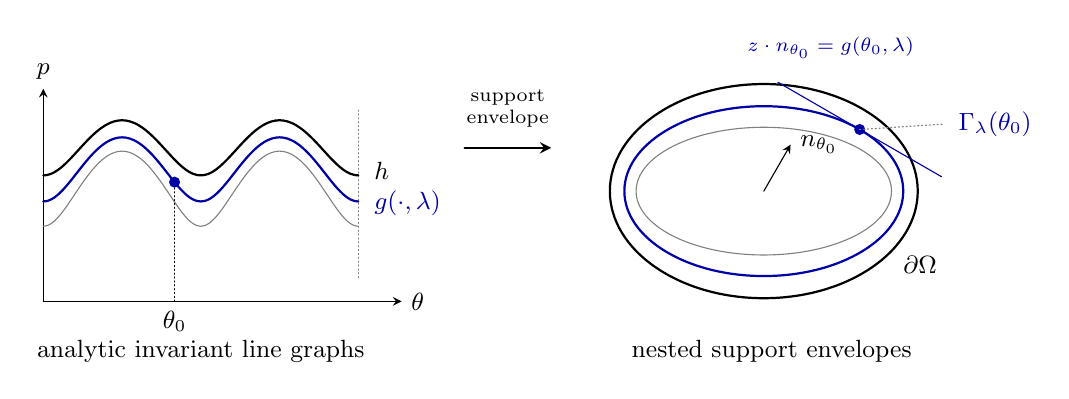
\begin{tikzpicture}[font=\small,>=stealth,line cap=round]
  \pgfmathsetmacro{\selectedsupport}{sqrt(4.34*cos(60)^2+1.61*sin(60)^2)}
  \pgfmathsetmacro{\contactx}{.85*4.34*cos(60)/\selectedsupport}
  \pgfmathsetmacro{\contacty}{.85*1.61*sin(60)/\selectedsupport}
  \begin{scope}
    \draw[->] (0,0)--(4.55,0) node[right] {$\theta$};
    \draw[->] (0,0)--(0,2.7) node[above] {$p$};
    \draw[densely dotted,gray] (4,.3)--(4,2.45);
    \draw[thick,domain=-90:270,samples=81,smooth,variable=\a]
      plot ({(\a+90)/90},{sqrt(5.29*cos(\a)^2+2.56*sin(\a)^2)});
    \draw[blue!65!black,thick,domain=-90:270,samples=81,smooth,variable=\a]
      plot ({(\a+90)/90},{sqrt(4.34*cos(\a)^2+1.61*sin(\a)^2)});
    \draw[gray,domain=-90:270,samples=81,smooth,variable=\a]
      plot ({(\a+90)/90},{sqrt(3.64*cos(\a)^2+.91*sin(\a)^2)});
    \node[anchor=west] at (4.08,1.66) {$h$};
    \node[anchor=west,blue!65!black] at (4.08,1.25) {$g(\cdot,\lambda)$};
    \draw[densely dotted] (1.6667,0)--(1.6667,\selectedsupport);
    \fill[blue!65!black] (1.6667,\selectedsupport) circle (2pt);
    \node[below] at (1.6667,0) {$\theta_0$};
    \node at (2,-.63) {analytic invariant line graphs};
  \end{scope}
  \draw[->,thick] (5.35,1.95)--(6.45,1.95);
  \node[align=center,font=\scriptsize] at (5.9,2.45) {support\\envelope};
  \begin{scope}[xshift=9.15cm,yshift=1.4cm]
    \draw[thick] (0,0) ellipse [x radius=1.955,y radius=1.36];
    \draw[blue!65!black,thick] (0,0)
      ellipse [x radius=1.77076,y radius=1.07853];
    \draw[gray] (0,0) ellipse [x radius=1.62173,y radius=.81086];
    \draw[blue!65!black]
      ({\contactx-1.2*cos(150)},{\contacty-1.2*sin(150)})--
      ({\contactx+1.2*cos(150)},{\contacty+1.2*sin(150)});
    \fill[blue!65!black] (\contactx,\contacty) circle (2pt);
    \draw[gray,thin,densely dotted] (\contactx,\contacty)--(2.27,.85);
    \node[anchor=west,blue!65!black] at (2.35,.85)
      {$\Gamma_\lambda(\theta_0)$};
    \node[anchor=south,blue!65!black,font=\scriptsize] at (.85,1.56)
      {$z\cdot n_{\theta_0}=g(\theta_0,\lambda)$};
    \draw[->] (0,0)--(.34,.59) node[right] {$n_{\theta_0}$};
    \node[anchor=west] at (1.65,-.93) {$\partial\Omega$};
    \node at (.1,-2.03) {nested support envelopes};
  \end{scope}
\end{tikzpicture}
\caption{The support-envelope correspondence, drawn schematically.
The highlighted point of $p=g(\theta,\lambda)$ specifies the blue
tangent line on the right; its contact point is
$\Gamma_\lambda(\theta_0)=g n_{\theta_0}+g_\theta e_{\theta_0}$,
with $g$ and $g_\theta$ evaluated at $(\theta_0,\lambda)$.
Positive $g+g_{\theta\theta}$ makes each envelope strictly convex,
and $g_\lambda<0$ makes the family strictly nested.}
\label{fig:phase-to-caustic}
\end{figure}


Each \(K_\lambda\) is a compact convex body with nonempty interior:
it contains a disk about the origin of radius
\(\min_\theta g(\theta,\lambda)>0\), and the constraint with normal
\(z/|z|\) bounds \(|z|\) by \(\max_\theta g(\theta,\lambda)\).
Moreover \(K_0=\overline\Omega\), by the definition of \(h\).

We verify directly that \(\Gamma_\lambda\) is the whole boundary and
has support function \(g(\cdot,\lambda)\). Differentiation gives
\begin{equation}\label{phys:normal-parametrization}
 \Gamma_\lambda'(\theta)=\rho(\theta,\lambda)e_\theta.
\end{equation}
For a fixed angle \(\alpha\),
\[
 \frac{\dd}{\dd\theta}
   \bigl(\Gamma_\lambda(\theta)\cdot n_\alpha\bigr)
 =\rho(\theta,\lambda)\sin(\alpha-\theta).
\]
This projection has its unique maximum, modulo \(2\pi\), at
\(\theta=\alpha\), where its value is \(g(\alpha,\lambda)\).
Hence every point \(\Gamma_\lambda(\theta)\) satisfies all the
constraints defining \(K_\lambda\), with equality for its own normal,
and belongs to \(\partial K_\lambda\).

Conversely, let \(z\in\partial K_\lambda\).
The continuous nonnegative function
\(g(\theta,\lambda)-z\cdot n_\theta\) must vanish somewhere: a positive
minimum would place a disk about \(z\) inside \(K_\lambda\).
At a zero \(\alpha\), its derivative also vanishes. Thus
\[
 z\cdot n_\alpha=g(\alpha,\lambda),\qquad
 z\cdot e_\alpha=g_\theta(\alpha,\lambda),
\]
which gives \(z=\Gamma_\lambda(\alpha)\).
The unique-maximum property proves that this parametrization is
one-to-one on \(\T\); \eqref{phys:normal-parametrization} makes it
regular. Each support line has exactly one contact point, so the
boundary contains no nontrivial line segment and the body is strictly
convex. In fact its curvature is \(1/\rho>0\).
All these curves are real analytic.

The last inequality in \eqref{phys:support-inequalities} gives, for
\(0\leq\lambda<\mu\leq\lambda_0\),
\[
 g(\theta,\mu)\leq g(\theta,\lambda)-c_0(\mu-\lambda)
 \quad\hbox{for every }\theta.
\]
It follows that \(K_\mu\) is contained in the interior of \(K_\lambda\),
with a uniform positive gap between them. In particular the boundaries
are pairwise disjoint, and \(\Gamma_\lambda\subset\Omega\) for
\(\lambda>0\).

The positively oriented tangent at \(\Gamma_\lambda(\theta)\) has
velocity \(e_\theta\) and line equation
\(z\cdot n_\theta=g(\theta,\lambda)\).
For \(\lambda>0\) these are precisely the line states in
\eqref{phys:invariance}, with \(t=\sqrt\lambda\).
They meet \(\Omega\), because their contact points lie in its interior.
The onto invariance in \eqref{phys:invariance} therefore preserves
tangency under both \(T\) and \(T^{-1}\). It supplies the tangent
successor segment at the forward endpoint and the tangent predecessor
segment at the back endpoint. Reflection is a linear involution:
if \(v'\) is the reflection of \(v\), then \(-v\) is the reflection
of \(-v'\). Reversing each such pair of segments proves tangency
preservation for the opposite orientation as well. Thus every positive
leaf is a smooth closed convex caustic, with the required reflection
property at either endpoint.

It remains to show that these curves fill a physical collar.
The map
\[
 F:\T\times[0,\lambda_0]\longrightarrow\overline\Omega,
 \qquad F(\theta,\lambda)=\Gamma_\lambda(\theta),
\]
is continuous and injective, by simplicity of the curves and strict
nesting. Since its domain is compact, it is a homeomorphism onto its
image. Set
\[
 A=K_0\setminus K_{\lambda_0}.
\]
This is relatively open in \(K_0=\overline\Omega\) and contains
\(\partial\Omega\). All leaves with \(\lambda<\lambda_0\) lie in \(A\).
For the converse, fix \(z\in A\) and consider its minimum support slack
\[
 m_z(\lambda)
   =\min_{\theta\in\T}
      \bigl(g(\theta,\lambda)-z\cdot n_\theta\bigr).
\]
This function is continuous, satisfies
\(m_z(0)\geq0>m_z(\lambda_0)\), and obeys
\[
 m_z(\mu)\leq m_z(\lambda)-c_0(\mu-\lambda)
 \qquad(\mu>\lambda).
\]
It has exactly one zero in \([0,\lambda_0)\).
At that zero, \(z\in\partial K_\lambda\), hence
\(z=\Gamma_\lambda(\theta)\) for exactly one \(\theta\).
The restriction of \(F\) to \(\T\times[0,\lambda_0)\) is therefore a
homeomorphism onto \(A\). Rescaling \(\lambda=b\lambda_0\) completes
the proof.
\end{proof}

\begin{proof}[Proof of Theorem~\ref{thm:collar-regularity}]
Theorem~\ref{thm:analytic-boundary} proves that the billiard boundary
is real analytic. Theorem~\ref{thm:joint} and
Proposition~\ref{prop:physical-collar} give the asserted jointly
real-analytic family of strictly convex caustics and its full
physical collar.
\end{proof}

\begin{proof}[Proof of Theorem~\ref{thm:main}]
Proposition~\ref{prop:physical-collar} gives exactly the continuous
caustic collar of \cite[Definition~1.1]{NB}: the boundary is the zero
leaf, the positive leaves are smooth closed convex caustics, and the
family parametrizes a relatively open neighborhood of the boundary
in the closed table. The original assumptions supply the remaining
smoothness, strict convexity, and positive curvature hypotheses.
Theorem~\ref{thm:nb-rigidity}, namely \cite[Theorem~1.2]{NB},
therefore implies that \(\Omega\) is an ellipse. Undoing the initial
translation gives a center \(c\in\R^2\) and a real symmetric
positive-definite matrix \(Q\) with
\[
 \Omega=\{x\in\R^2:(x-c)^TQ(x-c)<1\},
\]
as required.
\end{proof}


\begingroup
\small
\raggedright
\setlength{\bibsep}{5pt}
\bibliographystyle{plainnat}
\bibliography{references}
\endgroup
\end{document}
